% \chapter{Forward and Inverse Kinematics}\label{chap:kinematics}
\chapter{正运动学和逆运动学}
\label{chap:kinematics}

% In order to plan a robot's movements, we have to understand the relationship between the actuators that we can control and the robot's resulting position in the environment. For static arms, this is rather straightforward: if we know the position/angle of each joint, we can calculate the position of its end-effectors using trigonometry. This process is known as \emph{forward kinematics}. \index{Forward Kinematics} If we want to calculate the position each joint needs to be at, we need to invert this relationship. This is known as inverse kinematics. \index{Inverse Kinematics} For mobile robots, this process is usually more involved, as speeds need to be integrated, which we refer to as \emph{odometry}\index{Odometry}.

为了规划机器人的运动,我们必须了解我们可以控制的驱动器与机器人在环境中的所得位置之间的关系。对于静态操作臂,这是相当简单的:如果我们知道每个关节的位置/角度,我们可以使用三角法来计算其末端执行器的位置。这个过程称为\emph{正运动学}。\index{正运动学}如果我们知道末端执行器的位置,要计算每个关节所需的位置,我们需要反转这种关系。 这被称为逆运动学。\index{逆运动学}因为需要考虑速度,移动机器人通常会更多地涉及到这个过程,我们称之为\emph{里程计(Odometry)}\index{里程计(Odometry)}。

% The goals of this chapter are:
本章的目标是:

% \begin{itemize}
% \item introduce coordinate systems and their transformations,
% \item to introduce the forward kinematics of simple arms and mobile robots
% \item understand the concept of holonomy,
% \item show how solutions for the inverse kinematics for both static and mobile robots can be derived,
% \item provide an intuition on the relationship between inverse kinematics and path-planning.
% \end{itemize}

\begin{itemize}
\item 介绍坐标系及其变换
\item 介绍简单操作臂和移动机器人的正运动学
\item 了解整体的概念
\item 介绍如何推导静态机器人和移动机器人的逆运动学
\item 理解逆运动学和路径规划之间的关系
\end{itemize}

% \section{Coordinate Systems and Frames of Reference}\label{sec:coordsystems}
\section{坐标系和参考系}\label{sec:coordsystems}
\screencast{http://youtu.be/klBJi-MEeNQ}{coordinatesystem}

% Every robot assumes a position in the real world that can be described by its position (x, y and z) and orientation (pitch, yaw and roll) along the three major axes of a Cartesian Coordinate system (See also Section \ref{sec:dof}, ``Degrees of freedom''). Such a coordinate system is shown in Figure \ref{fig:coordinatesystem}. Note that the directions and orientations of the coordinate axes are arbitrary. This books uses the ``right hand rules'', which are illustrated in Figure \ref{fig:coordinatesystem} to determine axes labels and directions throughout. Pitch, yaw, and roll, are also known as bank, attitude, and heading in other communities. \index{Pitch}\index{Yaw}\index{Roll}\index{Bank}\index{Attitude}\index{Heading} This makes sense, considering the colloquial use of the word ``heading'', which corresponds to a rotation around the z-axis of a vehicle driving on the x-y-plane. 

假定每个机器人在现实世界中可以通过其位置(x,y和z)和沿笛卡尔坐标系的三个主轴的方向(俯仰,偏航和滚动)来描述其位姿(位置+姿态)(另见第\ref{sec:dof节},“自由度”)。坐标系如图\ref{fig:coordinatesystem}所示。 请注意,坐标轴的方向是任意的。这本书使用“右手法则”,它们如图\ref {fig:coordinatesystem}所示,以确定轴标签和方向。俯仰,偏航和滚动,在其他领域也被称为bank,attitude和heading。\index{Pitch}\index{Yaw}\index{Roll} \index{Bank} \index{Attitude} \index{Heading}因为生活中我们用“heading”来表达行驶的车辆围绕$xy$平面上的$z$轴的旋转,所以这是可以理解的。

\begin{figure}
	\centering
		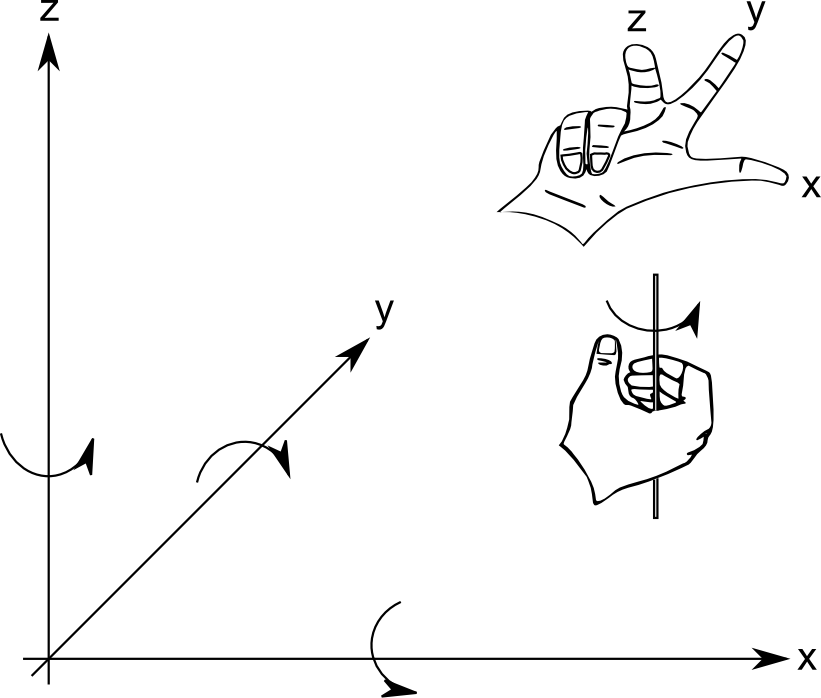
\includegraphics[width=0.8\textwidth]{figs/coordinatesystem}
	\caption{带有坐标轴和围绕它们的旋转的方向指示的坐标系。 这些方向是使用“右手法则”得出的。}
	% \caption{A coordinate system indicating the directions of the coordinate axes and rotation around them. These directions have been derived using the right-hand rules.}
	\label{fig:coordinatesystem}
\end{figure}

% Defining all three position axes and orientations might be cumbersome. What level of detail we care about, where the origin of this coordinate system is, and even what kind of coordinate system we chose, depends on the specific application. For example, a simple mobile robot would typically require a representation with respect to a room, a building, or the earth's coordinate system (given by the longitude and latitude of each point on the earth), whereas a static manipulator usually has the origin of its coordinate system at it's base. More complicated systems, such as mobile manipulators or multi-legged robots, make life much easier by defining multiple coordinate systems, e.g.\one for each leg and one that describes the position of the robot in the world frame. These local coordinate systems are known as \emph{Frames of Reference}\index{Frame of Reference}. 

定义所有三个位置轴和方向可能很麻烦。我们关心的是什么级别的细节,这个坐标系的原点,甚至是我们选择的什么样的坐标系,取决于具体的应用。 例如,简单的移动机器人通常需要相对于房间、建筑物或地球坐标系的表示(由地球上的每个点的纬度和纬度给出),而静态操作臂通常具有它的基准坐标系。 更复杂的系统,例如移动操作臂或多足机器人,定义多个坐标系更方便,例如每条腿一个坐标系加上机器人在世界中的位置的坐标系。这些局部坐标系称为\emph{参考系}\index {参考系}。

% An example of two nested coordinate systems is shown in Figure \ref{fig:nestedcoords}. In this example, a robot located at the origin of $x',y'$ and $z'$ might plan its motions in its own reference frame, which can then be expressed in the coordinate system $x$, $y$ and $z$ by performing a translation and a rotation as we will later see. 

图\ref{fig:nestedcoords}是两个嵌套坐标系的例子。 在这个例子中,位于$ x'$,$y'$和$ z'$原点的机器人可以在自己的参考系中规划其运动,然后可以通过执行位移和旋转在坐标系$ x $,$ y $和 $ z $中表示,我们稍后会讲到。

% Depending on it's degrees-of-freedom, that is the number of independent translations and rotations a robot can achieve in Cartesian space, it is also customary to ignore components of position and orientation that remain constant. For example a simple floor-cleaning robot's pose might be completely defined by it's $x$ and $y$ coordinates in a room as well as its orientation, i.e.\its rotation around the $z$-axis. 

根据机器人的自由度(也就是机器人可以在笛卡尔空间中独立位移和旋转的数量),通常我们会忽略保持不变的位置和方向的组件。例如,一个简单的地板清洁机器人的姿态可以完全定义为它在一个房间内的$ x $和$ y $坐标以及它的方向,即它围绕$ z $轴旋转。

\begin{figure}
	\centering
		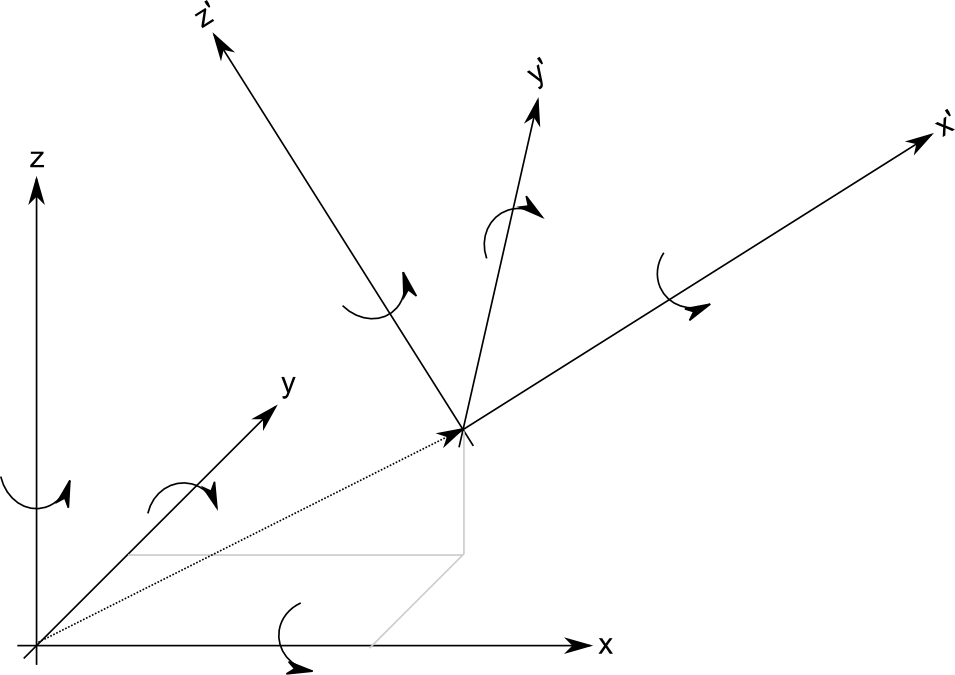
\includegraphics[width=\textwidth]{figs/frameofreference.png}
	% \caption{Two nested coordinate systems (frames of reference).}
	\caption{两个嵌套坐标系(参考系)。}
	\label{fig:nestedcoords}
\end{figure}

% \subsection{Matrix notation}
\subsection{矩阵符号}

% Given some kind of fixed coordinate system, we can describe the \emph{position} of a robot's end-effector by a $3x1$ position vector. As there can be many coordinate systems defined on a robot and the environment, we identify the coordinate system a point relates to by a preceeding super-script, e.g., $ ^AP$ to indicate that point $P$ is in coordinate system $\{A\}$. Each point consists of three elements $ ^AP=[p_x p_y p_z]^T$.

给定某种固定坐标系,我们可以用$ 3\times 1 $的位置向量来描述机器人末端驱动器的\emph {位置}。 由于可以在机器人和环境中定义许多坐标系,所以我们通过一个先前的超级脚本来确定一个点所涉及到的坐标系,例如$ ^AP $来表示点$ P $是坐标系$\{A\}$中一点。 每个点由三个元素组成:$ ^AP = [p_x p_y p_z]^T $。

% More formally, $^AP$ is a linear combination of the three basis vectors that span $A$:
更正式地,$ ^ AP $是定义在坐标系$A$中的三个基本向量的线性组合:
\begin{equation}
^AP=p_x\left(\begin{array}{c}1\\0\\0\end{array}\right)+p_y\left(\begin{array}{c}0\\1\\0\end{array}\right)+p_z\left(\begin{array}{c}0\\0\\1\end{array}\right)\label{eq:basis}
\end{equation}

\screencast{http://youtu.be/QdHO_9M8-UI}{frameofreference}

% As we know, not only the position of the robot is important, but also its orientation. In order to describe the orientation of a point, we will attach a coordinate system to it. Let $ \hat{X}_B, \hat{Y}_B$ and $ \hat{Z}_B$ be unit vectors that correspond to the principal axes of a coordinate system $\{B\}$. When expressed in coordinate system $\{A\}$, they are denoted $^A\hat{X}_B, ^A\hat{Y}_B$ and $ ^A\hat{Z}_B$. In order to express a vector that is given in one coordinate system in another, we need to project each of its components to the unit vectors that span the target coordinate system. For example considering only the axis $^A\hat{X}_B$

我们知道,机器人的位置很重要,机器人的方向也很重要。为了描述一个点的方向,我们再加一个坐标系。令$\hat{X}_B$,$\hat{Y}_B$和$\hat{Z}_B$是对应于坐标系$\{B\}$的主轴的单位向量。当在坐标系$\{A\}$中表示时,它们被表示为$^A\hat{X}_B,^A\hat{Y}_B$和$^A\hat{Z}_B$。为了表达在另一个坐标系中给出的向量,我们需要将其每个分量投影到跨越目标坐标系的单位向量。例如只考虑$^A\hat{X}_B$轴。

\begin{equation}\label{eq:projection}
^A\hat{X}_B=(\hat{X}_B\cdot\hat{X}_A, \hat{X}_B\cdot\hat{Y}_A,\hat{X}_B\cdot\hat{Z}_A)^T
\end{equation}

% consists of the projections of $\hat{X}_B$ onto $\hat{X}_A$, $\hat{Y}_A$ and $\hat{Z}_A$. Here,  $|\cdot|$ denotes the scalar product (also known as dot or inner product).  Note that all vectors in (\ref{eq:projection}) are unit vectors, i.e. their length is one. By definition of the scalar product, $A\cdot B=\|A\|\|B\|\cos \alpha=\cos \alpha$, indeed reduces the projection of $\hat{X}_B$ onto the unit vectors of $\{A\}$. This projection is illustrated in Figure \ref{fig:projection}.

包括$\hat{X}_B$到$\hat{X}_A$,$\hat{Y}_A$和$\hat{Z}_A$的投影。这里,$|\cdot|$表示标量积(也称为点积或内积)。注意,(\ref{eq:projection})中的所有向量都是单位向量,即它们的长度是$1$。根据标量积的定义,$ A\cdot B =\|A\|\|B\|\cos \alpha=\cos\alpha$确实减少了$\hat{X}_B$到单元上的投影$\{A\}$的向量。该投影如图\ref{fig:projection}所示。

\begin{figure}
	\centering
	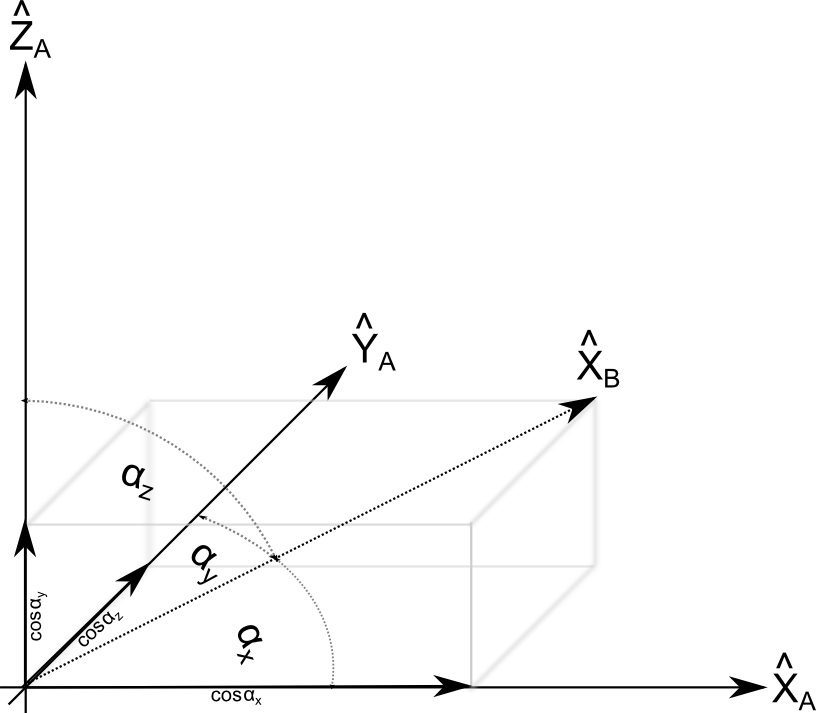
\includegraphics[width=0.8\textwidth]{figs/projection.png}
	% \caption{Top: A coordinate system $\{B\}$ with position given by $^AP$ and orientation given by $\hat{X}_B$, $\hat{Y}_B$, and $\hat{Z}_B$. Bottom: The projection of the unit vector $\hat{X}_B$ onto the unit vectors that span coordinate system $\{A\}$ after moving $\{B\}$ into the origin of $\{A\}$. As all vectors are unit vectors, $A\cdot B=\|A\|\|B\|\cos \alpha=\cos \alpha$. }
	\caption{上图:坐标系$\{B\}$,位置由$^AP$和由$\hat{X}_B$,$\hat{Y}_B$和$\hat{Z}_B$。下图:将$\{B\}$移动到$\{A\}$的原点后,将单位向量$\hat{X}_B$投影到跨越坐标系$\{A\}$的单位向量上。由于所有向量都是单元向量,因此$A\cdot B=\|A\|\|B\|\cos\alpha=\cos\alpha$。}
	\label{fig:projection}
\end{figure}

% We can now do this for all three vectors that span coordinate system $\{B\}$ and stack these three vectors together into a 3x3 matrix to obtain the rotation matrix

我们现在可以对跨越坐标系$\{B\}$的所有三个向量执行此操作,并将这三个向量一起堆叠成$3\times3$矩阵以获得旋转矩阵

%
\begin{equation}
^A_BR=[^A\hat{X}_B \quad ^A\hat{Y}_B \quad ^A\hat{Z}_B]
\end{equation}
%
% which describes $\{B\}$ relative to $\{A\}$. It is important to note that all columns in $ ^A_BR$ are unit vectors, so that the rotation matrix is orthonormal. This is important as this allows us to easily obtain the inverse of $ ^A_BR$ as $ ^A_BR^T$ or $ ^B_AR=^A_BR^T$. 

其中描述$\{B\}$相对于$\{A\}$。重要的是要注意,$^A_BR$中的所有列都是单位向量,因此旋转矩阵是正交的。这很重要,因为这样我们可以很容易地获得$^A_BR$的逆$A_BR^T$或$^B_AR=^A_BR^T$。

% Why the unit vectors of a coordinate system $\{B\}$ expressed in coordinate system $\{A\}$ actually make up a rotation matrix, can be easily seen when re-arranging equation \ref{eq:basis} in matrix form

为什么在坐标系$\{A\}$中表示的坐标系$\{B\}$的单位向量实际上构成一个旋转矩阵,当重新以矩阵形式排列等式\ref{eq:basis}时,就可以很容易地发现

\begin{equation}
^AP=\left(\begin{array}{ccc}1 & 0 & 0\\0 & 1 & 0\\0 & 0 & 1\end{array}\right)\left(\begin{array}{c}p_x\\p_y\\p_z\end{array}\right),
\end{equation}

% where the rotation matrix is nothing but the identity as both points already are in the same coordinate system. 

其中旋转矩阵不过是标识,因为两个点已经在同一坐标系中。

% We have now established how to express the orientation of a coordinate system using a rotation matrix. Usually, coordinate systems don't lie on top of each other, but are also displaced from each other. Together, position and orientation is known as a \emph{frame},\index{Frame} which is a set of four vectors, one for the position and three for the orientation, and we can write
%

我们现在已经解释了如何使用旋转矩阵来表达坐标系的方向。 通常,坐标系不能互相排列,而应相互偏离。 位置和方向一起被称为\emph{frame},\index {Frame},它是四个向量的集合,一个用于表示位置,三个表示用于方向,我们可以写成

\begin{equation}
\{B\}=\{^A_BR, ^AP\}
\end{equation}
%
% to describe the coordinate frame $\{B\}$ with respect to $\{A\}$ using a vector $^AP$ and a rotation matrix $^A_BR$. Robots usually have many such frames defined along their bodies.

使用向量$^AP$和旋转矩阵$^A_BR$来描述$\{A\}$的坐标系$\{B\}$。 机器人通常沿着它们的身体定义许多这样的坐标系。

% \subsection{Mapping from one frame to another}
\subsection{从一个坐标系映射到另一个坐标系}
\screencast{http://youtu.be/NsiJNvsuO3s}{rotationmatrix}

% Having introduced the concept of frames, we need the ability to map coordinates in one frame to coordinates in another frame. For example, lets consider frame $\{B\}$ having the same orientation as frame $\{A\}$ and sitting at location $^AP$ in space. As the orientation of both frames is the same, we can express a point $ ^BQ$ in frame $\{A\}$ as

引入了坐标系的概念后,我们需要能够将一坐标系中的坐标映射到另一坐标系中的坐标。 例如,让我们考坐标系$ \{B \} $与坐标系$ \{A \} $方向一致,并且位于$ ^ AP $。 由于两坐标系的方向是一样的,我们可以点$ ^ BQ $表示为坐标系$ \{A \} $中一个点

%
\begin{equation}
^AQ=^BQ+^AP
\end{equation}
%
% Actually, adding two vectors that are in different reference frames, i.e., $ ^BQ+^AP$, is only possible if both of them have the same orientation. We can, however, convert from one reference frame to the other using the rotation matrix:

实际上,只有两个参考坐标系中的两个向量方向相同,者两个向量才可以做加法,即$ ^ BQ + ^ AP $。然而,我们可以通过旋转矩阵将一个参考坐标系转换到另一个参考坐标系:

\begin{equation}
^AP=^A_BR^BP
\end{equation}
%
% and therefore solve the mapping problem regardless of the orientation of $\{A\}$ to $\{B\}$:

因此无论$\{A\}$到$ \{B\} $的方向如何我们都可以解决映射问题:

\begin{equation}
^AQ=^A_BR^BQ+^AP
\end{equation}
% Using this notation, we can see that leading subscripts cancel the leading superscripts of the following vector/rotation matrix. Whereas we have now a solution to transfer a point from one frame of reference to another by combining a rotation and a translation, it would be more appealing to write something like that:

使用这个符号,我们可以看到,引导下标取消了以下向量/旋转矩阵的前导上标。现在我们已经可以通过位移和旋转来将一个点从一个坐标系转换到另一坐标系上。如果能写成如下形式会更好些:

\begin{equation}
^AQ=^A_BT^BQ
\end{equation}
% In order to do this, we need to introduce a 4x1 position vector such that

为了做到这一点,我们需要引入一个$4\times1$的位置向量

\begin{equation}
\left[\begin{array}{c}^AQ\\\end{array}\right]=\left[\begin{array}{ccc|c} & ^A_BR & & ^AP \\\hline 0 & 0 & 0 & 1\end{array}\right]\left[\begin{array}{c}^BQ\\1\end{array}\right]
\end{equation}
% and $^A_BT$ is a 4x4 matrix.  Note that the added `1`s and $ [0 0 0 1]$ do not affect the other entries in the matrix during matrix multiplication. A 4x4 matrix of this form is called a \emph{homogenous transform}.\index{Homogenous Transform}

而$ ^A_BT$是一个$4\times 4$矩阵。 请注意,在矩阵乘法期间,添加的“1”和$ [0 0 0 1] $不会影响矩阵中的其他项。 这种形式的$4\times 4$矩阵称为\emph{齐次变换}。\index{齐次变换}

% The inverse of an homogeneous transform can be constructed by inverting rotation and translation part independently, leading to

可以通过独立地反向旋转和位移来构造齐次变换的逆,从而有

\begin{equation}
\left[\begin{array}{ccc|c} & ^A_BR & & ^AP \\\hline 0 & 0 & 0 & 1\end{array}\right]^{-1}=
\left[\begin{array}{ccc|c} & ^A_BR^T & & -^A_B{R^T}{^AP} \\\hline 0 & 0 & 0 & 1\end{array}\right]
\end{equation}

% We have now established a convenient notation to convert points from one coordinate system to another. There are many possible ways this can be done, in particular how rotation can be represented (see below), but all can be converted from one into the other. 

我们现在已经建立了一个便捷的符号,将点从一个坐标系转换到另一个坐标系。存在许多其它的方法,特别是表示旋转(见下文),但是它们之间可以相互转换。

% \subsection{Transformation arithmetic}
\subsection{变换算术}
% Transformations can be combined: consider for example an arm with two links, reference frame $\{A\}$ at the base, $ \{B\} $ at its first joint, and $\{C\}$ at its end-effector. Given the transforms $ ^B_CT$ and $ ^A_BT$, we can write

可以组合变换:例如具有两个链的手臂,基座参坐标系$ \{A \} $,其第一个关节处的坐标系$ \{B\} $和其末端执行器的坐标系$ \{C\} $。 给定转换$ ^ B_CT $和$ ^ A_BT $,我们可以用

\begin{equation}
^AP=^A_BT^B_CT^CP=^A_CT^CP
\end{equation}
% to convert a point in the reference frame of the end-effector to that of its base. As this works for rotation and translation operators independently, we can construct $ ^A_CT$ as

来把末端执行器参考系中的一个点转换为其基座参考系的一点。因为这分别适用于旋转和位移,我们可以将$ ^A_CT $构造为

\begin{equation}
^A_CT=\left[\begin{array}{ccc|c} & ^A_BR^B_CR & & ^A_BR^BP_C +^AP_B \\\hline 0 & 0 & 0 & 1\end{array}\right]
\end{equation}
%
% where $ ^AP_B$ and $ ^BP_C$ are the translations from $\{A\}$ to $\{B\}$ and from $ \{B\}$ to $\{C\}$, respectively.

其中$ ^AP_B $和$ ^BP_C $分别是从$ \{A\} $到$ \{B\} $和从$ \{B\} $到$ \{C\} $的位移。

% \subsection{Other representations for orientation}
\subsection{其他的方向表示}

% So far, we have represented orientation by a 3x3 matrix who's column vectors are orthogononal unit vectors describing the orientation of a coordinate system. Orientation is therefore represented with nine different values. We chose this representation mainly because it is the most intuitive to explain and is derived from simple geometry.

到目前为止,我们已经通过3x3矩阵来表示方位,列向量是描述坐标系方位的正交单位向量。 因此,方向由九个不同的值表示。 我们选择了这个表示,主要是因为它是最直观的解释,而是从简单的几何派生出来的。

% In fact, three values are sufficient to describe orientation. This becomes clear when considering that orthogonality (dot product of all columns is zero) and vector length (each vector must have length 1) impose six constraints on the nine values in the rotation matrix. Indeed, an orientation can be represented about a rotation by certain angles around the $x$, the $y$, and the $z$-axis of the reference coordinate system. This is known as the $X-Y-Z$ fixed angle notation.\index{Fixed angle notation} Mathematically, this can be represented by a rotation matrix of the form

事实上,三个值足以描述方向。 当考虑到正交性(所有列的点积为零)和向量长度(每个向量必须具有长度1)时,在旋转矩阵中的九个值上施加六个约束,这变得清楚。 实际上,可以将参考坐标系的$ x $,$ y $和$ z $ -axis周围的某个角度的旋转表示为方向。 这被称为$ X-Y-Z $固定角度符号。\index {固定角度符号}数学上,这可以由表单的旋转矩阵

\begin{equation}
\tiny
^A_BR_{XYZ}(\gamma,\beta,\alpha)=\left[\begin{array}{ccc}cos\alpha & -sin\alpha & 0\\sin\alpha & \cos\alpha & 0\\0 & 0 & 1\end{array}\right]\left[\begin{array}{ccc}cos\beta& 0 & sin\beta\\0 & 1 & 0\\-sin\beta & 0 & cos\beta\end{array}\right]\left[\begin{array}{ccc}1 & 0 & 0 \\0 & cos\gamma & -sin\gamma\\0 & sin\gamma & cos\gamma\end{array}\right]
\end{equation}

% While the $X-Y-Z$ fixed angles approach expresses a coordinate frame using rotations with respect to the original coordinate frame, say $\{A\}$, another possible description is to start with a coordinate frame $\{B\}$ that is coincident with frame $\{A\}$, then rotate around the Z-axis with angle $ \alpha$, then the Y-axis with angle $ \beta$ and finally around the X-axis with angle $ \gamma$. This representation is called Z-Y-X Euler angles.\index{Euler angles}

而$ XYZ $固定角度方法表示使用相对于原始坐标系的旋转的坐标系,例如$ \{A \} $,另一种可能的描述是从坐标框$ \{B \} $开始, 坐标系$ \{A \} $一致,然后绕Z轴旋转,角度为$ \alpha $,然后以角度$ \beta $的Y轴旋转,最后绕X轴旋转角度$ \gamma $。 这个表示被称为Z-Y-X欧拉角。\index {欧拉角}

% As the coordinate axis do not necessarily need to be different, there are twelve possible valid combinations of sub-sequent rotations:

由于坐标轴不一定需要不同,所以有以下12个可能的有效组合次序旋转:

\begin{center}
XYX, XZX, YXY, YZY, ZXZ, ZYZ, XYZ, XZY, YZX, YXZ, ZXY and ZYX
\end{center}
% There are only twelve, as sub-sequent rotations around the same axis are not valid. Such rotations would not add any information, but are equivalent to a rotation by the sum of both angles. 

只有十二个,因为在同一轴周围的后续轮转无效。 这样的旋转不会增加任何信息,而是相当于两个角度之和的旋转。

% It is important to know about the subtle differences between the different available transformations as there is no ``right'' or ``wrong'', but different manufacturers and fields use different conventions. There is only one caveat: each of the rotation matrices can look like subsequent rotations around the same axis for certain values of angles. For example, this happens for the XYZ rotation matrix if the angle of rotation around the Y-axis is $90^o$. These cases are known as a \emph{singularity}\index{Singularity} .

知道不同的可用转换之间的微妙差异是重要的,因为没有“正确”或“错误”,但不同的制造商和领域使用不同的约定。 只有一个警告:每个旋转矩阵可以看起来像对于某些角度值围绕同一轴线的后续旋转。 例如,如果Y轴周围的旋转角为$ 90 ^ o $,则会发生XYZ旋转矩阵。 这些情况称为\emph {singularity} \index {Singularity}。

% Among these, the preferred representation for computational and stability reasons are \emph{Quaternions}\index{Quaternion}. A quaternion is a 4-tuple that extends the complex numbers with very general applications in mathematics and representing orientation and rotation in particular. The basic idea is that each rotation can be represented as a rotation around a single axis (a vector in space) by a specific angle. Given such an axis $ \hat{K}=[k_x k_y k_z]^T$ and an angle $ \theta$, one can calculate the so-called Euler parameters\index{Euler parameters} or unit quaternion\index{unit quaternion}:

其中,计算和稳定性原因的优选表示为\emph {Quaternions} \index {Quaternion}。 四元数是一个四元组,它将复数扩展为数学中非常普遍的应用,特别是表示取向和旋转。 基本思想是,每个旋转可以被表示为围绕单个轴的旋转(空间中的向量)特定的角度。 给定这样一个轴$ \hat {K} = [k_x k_y k_z]^ T $和一个角度$ \theta $,可以计算所谓的欧拉参数\index{欧拉参数}或单位四元数\index{单位四元数}:

\begin{eqnarray}
\epsilon_1=k_x sin \frac{\theta}{2}\\
\epsilon_2=k_y sin \frac{\theta}{2}\\
\epsilon_3=k_z sin \frac{\theta}{2}\\
\epsilon_4=cos\frac{\theta}{2}
\end{eqnarray}

These four quantities are constrained by the relationship
\begin{equation}
\epsilon_1^2+\epsilon_2^2+\epsilon_3^2+\epsilon_4^2=1
\end{equation}
% which might be visualized by a point on a unit hyper-sphere. %Transformations are represented by \emph{dual quaternions}\index{Dual quaternion}, one for the translation and one for the rotation. Dual quaternions can again easily be converted into homogenous transformation matrices.

这可能由单位超球体上的点可视化。

% Analogous to rotation matrices, two quaternions $\epsilon_i$ and $\epsilon_i'$ can be multiplied using the following equation

类似于旋转矩阵,可以使用以下等式乘以两个四元数$ \epsilon_i $和$ \epsilon_i'$

\begin{equation}
\left(
\begin{array}{cccc}
\epsilon_4 & \epsilon_1 & \epsilon_2 & \epsilon_3\\
-\epsilon_1 & \epsilon_4 & -\epsilon_3 & \epsilon_2\\
-\epsilon_2 & \epsilon_3 & \epsilon_4 & -\epsilon_1\\
-\epsilon_3 & -\epsilon_2 & \epsilon_1 & \epsilon_4
\end{array}{c}
\right)
\left(\begin{array}{c}\epsilon_4'\\\epsilon_1'\\\epsilon_2'\\\epsilon_3'\end{array}\right)
\end{equation}

% Unlike multiplying two rotation matrices, which requires 27 multiplications and 18 additions, multiplying two quaternions only requires 16 multiplications and 12 additions, making the operation computationally more efficient. In addition, the quaternion representation does not suffer from singularities for specific joint angles, making the approach computationally more robust. 

与需要27次乘法和18次加法的两个旋转矩阵相乘,乘以两个四元数只需要16次乘法和12次加法,使得运算在计算上更有效率。 此外,四元数表示法并不具有针对特定关节角度的奇异点,使得该方法在计算上更加鲁棒。

% Why any rotation can be expressed by a single vector can be seen when considering the properties of orthonomal rotation matrices. They have three Eigenvalues $\lambda=1$ and a complex pair $\lambda_{1,2}=\cos \theta \pm i \sin \theta$. Eigenvalues and Eigenvectors are defined as $Rv=\lambda v$. For the case of $\lambda=1$, the corresponding Eigenvector $v$ is unchanged by rotation. This is only possible if $v$ is the actual axis of rotation. The angle of rotation is now given by $\theta$, which can be inferred from the complex pair.  

为什么在考虑旋转旋转矩阵的性质时,可以看到单个向量可以表达出旋转。 他们有三个特征值$ \lambda = 1 $和复数对$ \lambda_ {1,2} = \cos \theta \pm i \sin \theta $。 特征值和特征向量定义为$ Rv = \lambda v $。 对于$ \lambda = 1 $的情况,相应的特征向量$ v $不变。 只有$ v $是实际的旋转轴才有可能。 旋转角度现在由$ \theta $给出,可以从复数对推断出。

% \section{Forward kinematics of selected Mechanisms}
\section{所选机制的正运动学}

% Now that we have introduced the notion of local coordinate frames, we are interested in how to calculate the pose and speed of these coordinate frames as a function of the robot's actuators. We will first consider simple mechanisms where we can determine the relationship between actuators and the pose of various frames on the robot both in the position and speed domain. We will then consider the special class of non-holonomous mechanisms using a series of wheeled robots, for which the forward kinematics can only be calculated in the speed domain. 

现在我们已经介绍了局部坐标系的概念,我们对于如何根据机器人的驱动器来计算这些坐标系的姿态和速度感兴趣。 我们将首先考虑简单的机制,我们可以在位置和速度域中确定驱动器与机器人各坐标系的姿态之间的关系。 然后,我们将考虑使用一系列轮式机器人的特殊类别的非全局机制,其中正运动学只能在速度域中计算。

\subsection{Forward kinematics of a simple arm}
\begin{figure}[!htb]%{L}{0.3\textwidth}
  \begin{center}
    \includegraphics[width=0.27\textwidth]{figs/fwk2dofarm}
  \end{center}
  % \caption{A simple 2-DOF arm.}
  \caption{简单的2自由度手臂}
  \label{fig:fwk2dofarm}
\end{figure}

% Consider a robot arm made out of two links and two joints that is mounted to a table. Let the length of the first link be $l_1$ and the length of the second link be $ l_2$. You could specify the position of the link closer to the table by the angle $ \alpha$ and the angle of the second link relative to the first link using the angle $ \beta$. Suitable conventions and coordinate systems are shown in Figure \ref{fig:fwk2dofarm}

考虑一个由两个连杆制成的机器人手臂和两个安装在桌子上的接头。 让第一个链接的长度为$ l_1 $,第二个链接的长度为$ l_2 $。 您可以使用角度$ \alpha $指定靠近桌面的链接的位置,并使用角度$ \beta $指定第二个链接相对于第一个链接的角度。 合适的惯例和坐标系如下图所示:\ref {fig:fwk2dofarm}

% We can now calculate the position of the joint between the first and the second link using simple trigonometry:

我们现在可以使用简单的三角学来计算第一和第二个链接之间的关节的位置:

\begin{eqnarray}\label{eq:cosxl1}
x_1 &=&\cos \alpha l_1\\
y_1 &=&\sin \alpha l_1
\end{eqnarray}

% Similarly, the position of the end-effector is given by
类似地,末端驱动器的位置由下式给出

\begin{eqnarray}
x_2&=&\cos(\alpha+\beta)l_2+x_1\\
y_2&=&\sin(\alpha+\beta)l_2+y_1
\end{eqnarray}
%
% or together, the position of the end-effector $(x,y)$ is given by
或者一起,终端驱动器$(x,y)$的位置由下式给出

\begin{eqnarray}\label{eq:cosx}
x&=&\cos(\alpha+\beta)l_2+\cos\alpha l_1\\
y&=&\sin(\alpha+\beta)l_2+\sin\alpha l_1
\end{eqnarray}

% The above equations are the kinematic equations of this robot as they relate its control parameters $ \alpha$ and $\beta$ to the position of its end-effector given in the local coordinate system spanned by $ x$ and $ y$ with the origin at the robot's base. Note that both $\alpha$ and $\beta$ shown in the figure are positive: Both links rotate around the z-axis. Using the right-hand rule, the direction of positive angles is defined to be counter-clockwise. 

上述等式是这个机器人的运动学方程,因为它们将控制参数$ \alpha $和$ \beta $与其在$ x $和$ y $之间的局部坐标系中给出的末端驱动器的位置相关联 起源于机器人的基地。 请注意,图中显示的$ \alpha $和$ \beta $均为正数:两个链接都绕z轴旋转。 使用右手规则,将正角度的方向定义为逆时针方向。

% The \emph{configuration space} \index{Configuration space}\index{C-Space (Configuration space)}, i.e., the set of angles each actuator can be set to, of this robot is given by $ \frac{-\pi}{2}<\alpha<\frac{\pi}{2}$ as it is not supposed to run into the table, and $ -\pi < \beta < \pi$. The configuration space is given with respect to the robot's joints and allows us to calculate the \emph{workspace}\index{Workspace} of the robot, i.e., the physical space it can move to, using the forward kinematic equations. This terminology will be identical for mobile robots. An example of configuration and work-space for both a manipulator and a mobile robot is shown in Figure \ref{fig:holonomy}.

\emph {configuration space} \index {配置空间} \index {C-Space(配置空间)},即每个驱动器可以设置为的角度的集合,由$ \frac { - \pi} {2} <\alpha <\frac {\pi} {2} $,因为它不应该进入表,而$ - \pi <\beta <\pi $。 给出了关于机器人关节的配置空间,并允许我们使用正运动学方程来计算机器人的\emph {workspace} \index {Workspace},即它可以移动的物理空间。 移动机器人的术语将是相同的。 机械手和移动机器人的配置和工作空间的一个例子如图\ref {fig:holonomy}所示。

% The orientation of the arm's end-effector is given by $\alpha+\beta$. We can now write down  a transformation that includes a rotation around the z-axis

手臂末端驱动器的方向由$ \alpha + \beta $给出。 现在我们可以写下一个围绕z轴旋转的转换

\begin{equation}
\label{eq:2armtrans}
\left(\begin{array}{llll}cos_{\alpha\beta} & -sin_{\alpha\beta} &  0 & \cos_{\alpha\beta}l_2+\cos\alpha l_1\\
                        sin_{\alpha\beta} & cos_{\alpha\beta} & 0 & \sin_{\alpha\beta}l_2+\sin\alpha l_1\\
												0 & 0 & 1 & 0\\
												0 & 0 & 0 & 1\end{array}\right)
\end{equation}
The notation $sin_{\alpha\beta}$ and $cos_{\alpha\beta}$ are short-hand for $sin(\alpha+\beta)$ and $cos(\alpha+\beta)$, respectively.

% This transformation now allows us to translate from the robot's base to the robot's end-effector as a function of the actuator positions $\alpha$ and $\beta$. This transformation will be helpful if we want to calculate suitable joint angles in order to reach a certain pose or if we want to convert measurements taken relative to the end-effector back into the base's coordinate system. 

这个转换现在允许我们根据驱动器位置$ \alpha $和$ \beta $的函数将机器人的基础转换为机器人的末端驱动器。 如果我们想要计算合适的关节角度以达到某个姿势,或者我们想将相对于末端驱动器的测量值转换回到基座的坐标系中,这种转换将会有所帮助。

% \subsection{Forward Kinematics of a Differential Wheels Robot}
\subsection{差速轮机器人的前进运动学}
\label{sec:fwkmobile}

% Whereas the pose of a robotic manipulator is uniquely defined by its joint angles---which can be made available using encoders in almost real-time---this is not the case for a mobile robot. Here, the encoder values simply refer to wheel orientation and need to be integrated over time, which will be a huge source of uncertainty as we will later see.

而机器人操作臂的姿态由关节角度唯一地定义,这可以使用编码器几乎实时地使用 - 这不是移动机器人的情况。 在这里,编码器值仅仅是指车轮定位,并且需要随着时间的推移而被集成,这将是我们稍后将看到的巨大的不确定性来源。

% What complicates matters is that for so-called \emph{non-holonomic} systems, it is not sufficient to simply measure the distance that each wheel traveled, but also when each movement was executed. 

重要的是,对于所谓的“非完整的”系统来说,简单地测量每个车轮行进的距离,而且每次执行时都是不够的。

\begin{figure}[htb!]
	\centering
		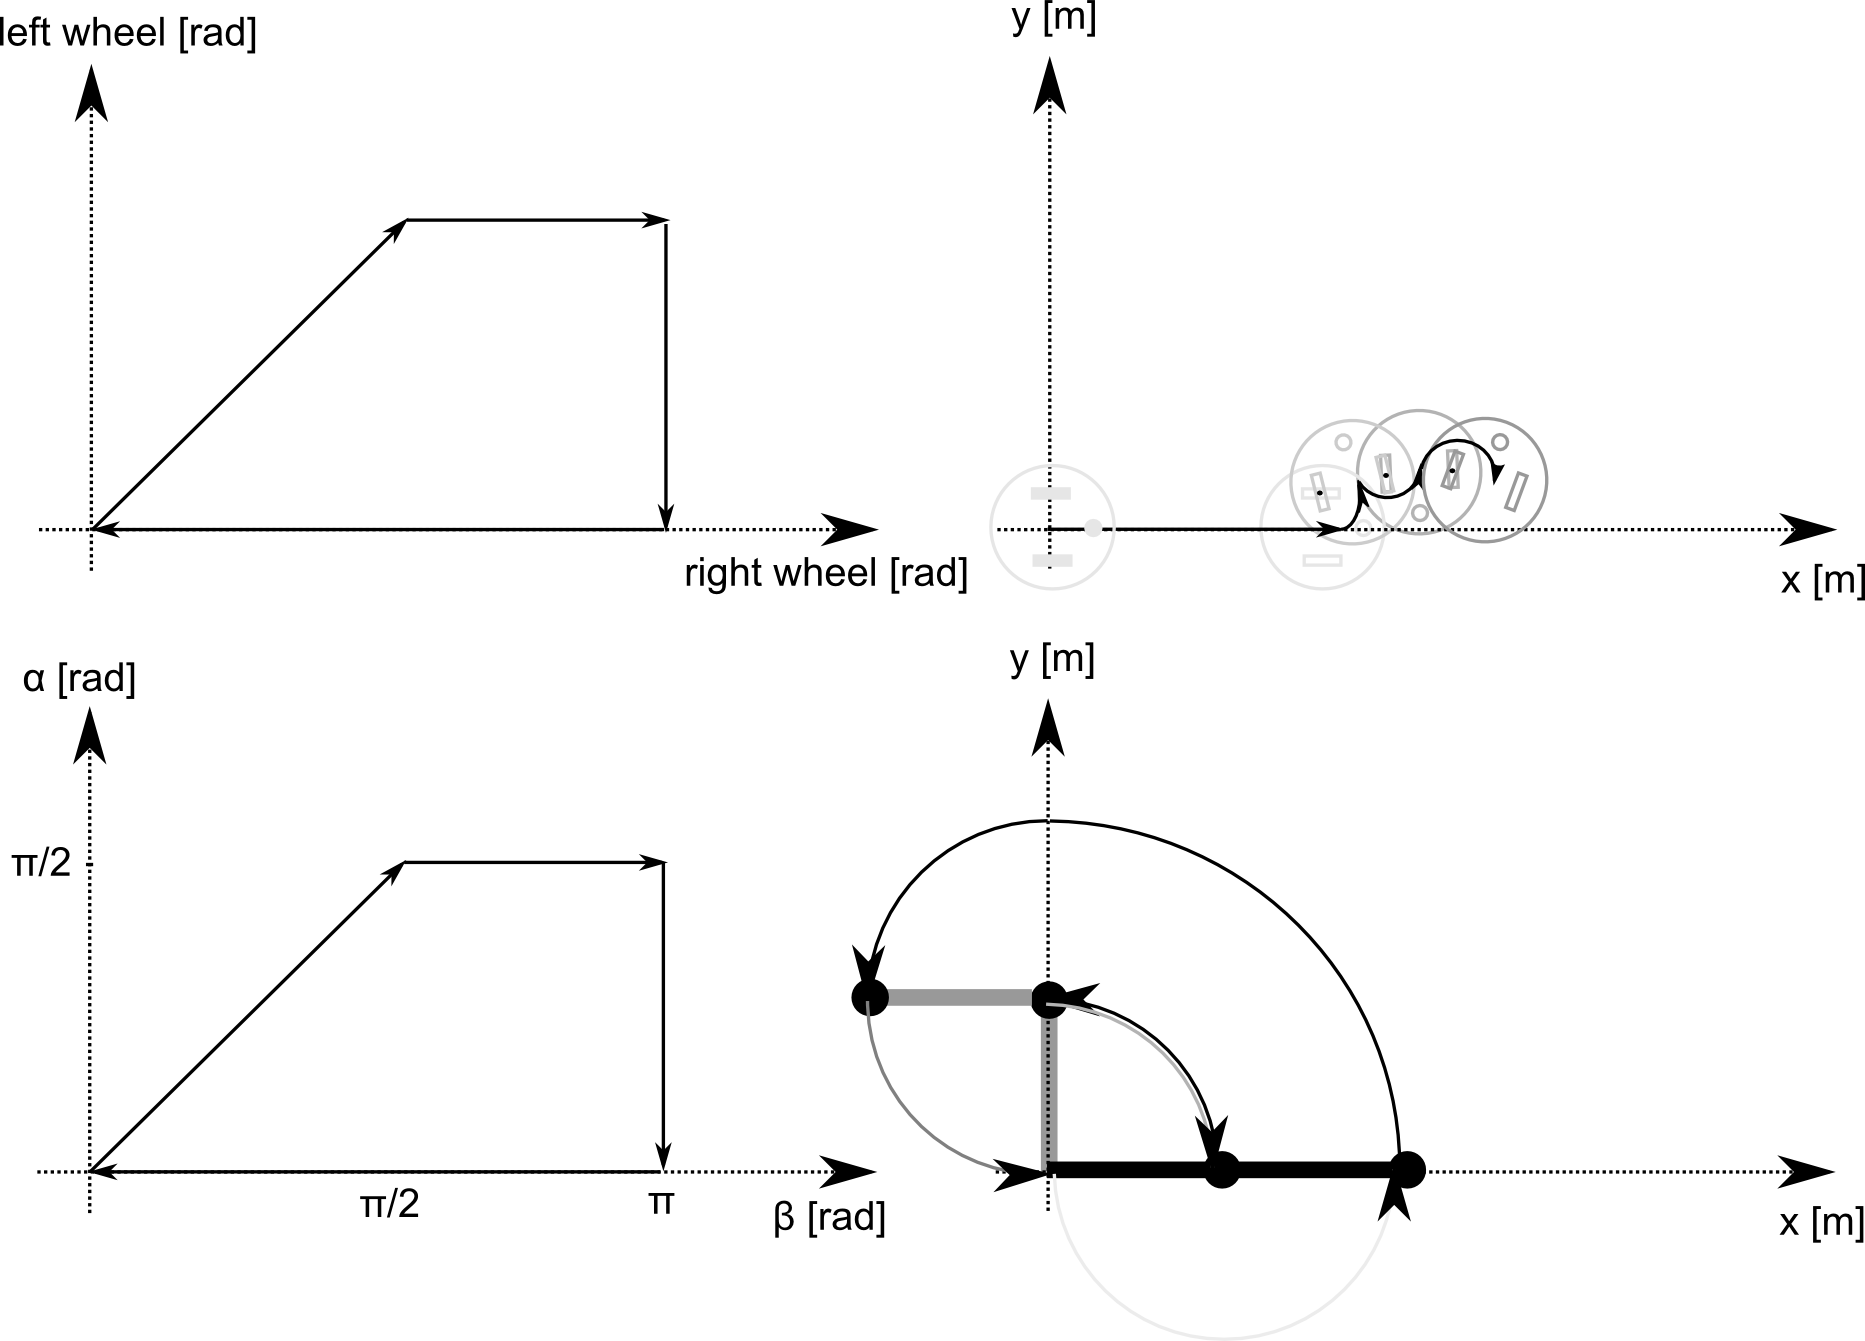
\includegraphics[width=0.95\textwidth]{figs/holonomy.png}
	% \caption{Configuration space (left) and workspace (right) for a non-holonomic mobile robot (top) and a holonomic manipulator (bottom). Closed trajectories in configuration space result in closed trajectories in the workspace if the robot's kinematics is holonomic.}
	\caption{非完整的移动机器人(上)和整体操作臂(底部)配置空间(左)和工作区(右)。 如果机器人的运动学是完整的,配置空间中的闭合轨迹会导致工作空间中的闭合轨迹。}
	\label{fig:holonomy}
\end{figure}

% A system is non-holonomic\index{Non-holonomic}\index{Holonomic} when closed trajectories in its configuration space (reminder: the configuration space of a two-link robotic arm is spanned by the possible values of each angle) may not have it return to its original state.  A simple arm is holonomic, as each joint position corresponds to a unique position in space. Going through whatever trajectory that comes back to the starting point in configuration space, will put the robot at the exact same position. A train on  a track is holonomic: moving its wheels backwards by the same amount they have been moving forward brings the train to the exact same position in space. A car and a differential-wheel robot are non-holonomic vehicles: performing a straight line and then a right-turn leads to the same amount of wheel rotation than doing a right turn first and then going in a straight line; getting the robot to its initial position requires not only to rewind both wheels by the same amount, but also getting their relative speeds right. The configuration and corresponding workspace trajectories for a non-holonomic and a holonomic robot are shown in Figure \ref{fig:holonomy}. Here, a robot first moves on a straight line (both wheels turn an equal amount). Then the left wheel remains fixed and only the right wheel turns forward. Then the right wheel remain fixed and the left wheel turns backward. Finally, the right wheel turns backward, arriving at the initial encoder values (zero). Yet, the robot does not return to its origin. Performing a similar trajectory in the configuration space of a two-link manipulator instead, let the robot return to its initial position. 

系统是非完整的\index {非完整} \index{完整}当其配置空间中的闭合轨迹(提醒:双链机器人臂的配置空间跨越每个角度的可能值)可能不让它回到原来的状态。一个简单的手臂是完整的,因为每个关节位置对应于一个独特的空间位置。通过任何返回到配置空间起点的轨迹,将机器人置于完全相同的位置。轨道上的火车是完整的:将车轮向后移动与前进的相同的数量使火车在太空中完全相同的位置。汽车和差速轮机器人是非完整的车辆:执行直线,然后右转导致与先行右转然后直线相同的车轮旋转量;使机器人达到初始位置不仅需要以相同的量倒转两个车轮,而且要使其相对速度正确。非完整和全面的机器人的配置和相应的工作空间轨迹如图\ref {fig:holonomy}所示。这里,机器人首先在直线上移动(两轮相等)。然后左轮保持固定,只有右轮向前转。然后右轮保持固定,左侧车轮向后转。最后,右轮转向,达到初始编码器值(零)。然而,机器人并没有回到起点。在双链机械手的配置空间中执行类似的轨迹,让机器人恢复到初始位置。

% It should be clear by now that for a mobile robot, not only traveled distance per wheel matters, but also the speed of each wheel as a function of time. Instead, this information was not required to uniquely determine the pose of a manipulating arm. Lets introduce the following conventions. We will establish a world coordinate system $\{I\}$, which is known as the inertial frame by convention (Figure \ref{fig:mobilerobot}). We establish a coordinate system $\{R\}$ on the robot and express the robot's speed $^R\dot{\xi}$ as a vector $ ^R\dot{\xi}=[^R\dot{x}, ^R\dot{y}, ^R\dot{\theta}]^T$. Here $^R\dot{x}$ and $^R\dot{y}$ correspond to the speed along the x and y directions in $\{R\}$, whereas $^R\dot{\theta}$ corresponds to the rotation around the imaginary z-axis, that you can imagine to be sticking out of the ground. We denote speeds with dots over the variable name, as speed is simply the derivative of distance.  Think about the robot's position in $\{R\}$ real quick. It is always zero, as the coordinate system is fixed on the robot. Therefore, velocities are the only interesting quantities in this coordinate system and we need to understand how velocities in $\{R\}$ map to positions in $ \{I\}$, which we denote by $^I\xi=[^Ix, ^Iy, ^I\theta]^T$. These coordinate systems are shown in Figure \ref{fig:mobilerobot}. 

现在应该清楚的是,对于移动机器人,不仅每轮行驶距离重要,而且每个车轮的速度也随着时间的推移而变化。相反,不需要这些信息来唯一地确定操纵臂的姿态。让我们介绍以下约定。我们将建立一个世界坐标系$ \{I \} $,这被称为惯例的惯坐标系(图\ref {fig:mobilerobot})。我们在机器人上建立一个坐标系$ \{R \} $,并将机器人的速度$ ^ R \dot{\xi} $作为向量$ ^R\dot{\xi} = [^R\dot{x},^R\dot{y},^R\dot{\theta}]^T $。这里$ ^R \dot {x} $和$ ^R \dot{y} $对应于$ \{R \} $中的x和y方向的速度,而$ ^R\dot{\theta} $对应于围绕虚拟z轴的旋转,您可以想象出将其伸出地面。我们用变量名称表示点的速度,因为速度只是距离的导数。想想机器人的位置在$ \{R \} $真正快速。当坐标系固定在机器人上时,它始终为零。因此,速度是这个坐标系中唯一有趣的数量,我们需要了解$ \{R \} $中的速度映射到$ \{I \} $中的位置,我们用$ ^ I\xi = [^Ix,^Iy,^I\theta]^T $。这些坐标系显示在图\ref{fig:mobilerobot}中。

\begin{figure}[htb!]
	\centering
		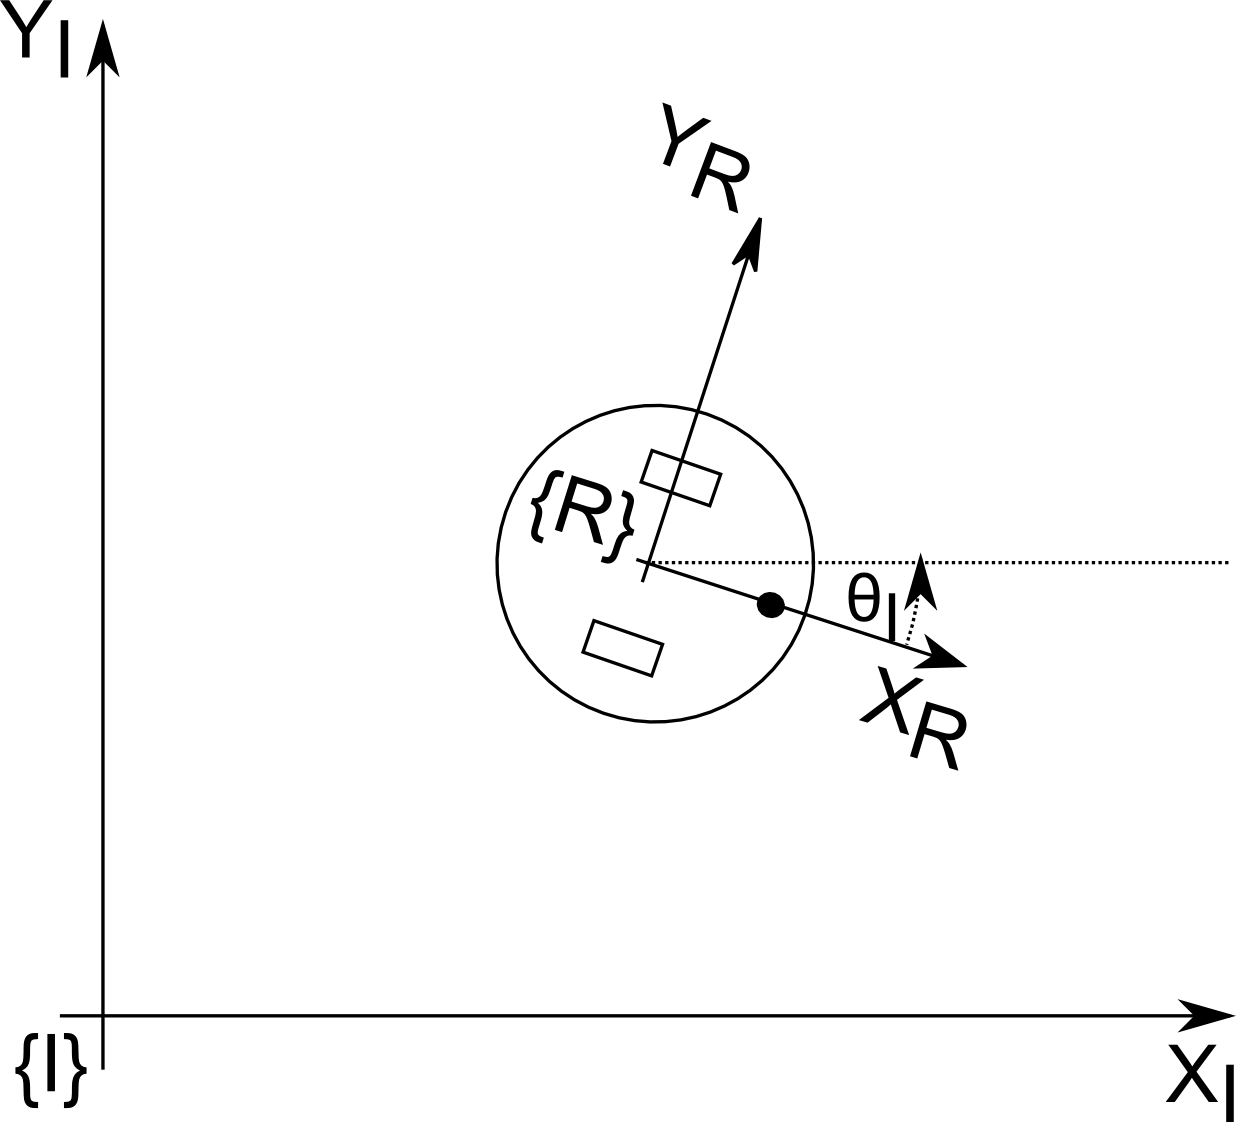
\includegraphics[width=0.85\textwidth]{figs/mobilerobot.png}
	% \caption{Mobile robot with local coordinate system \{R\} and world frame \{I\}. The arrows indicate the positive direction of position and orientation vectors.}
	\caption{具有局部坐标系\{R \}和世坐标系\{I \}的移动机器人。 箭头表示位置和方向向量的正方向。}
	\label{fig:mobilerobot}
\end{figure}

% Notice that the positioning of the coordinate frames and their orientation are arbitrary. Here, we chose to place the coordinate system in the center of the robot's axle and align $^Rx$ with its default driving direction.

请注意,坐标系的定位及其方向是任意的。 在这里,我们选择将坐标系放置在机器人轴的中心,并将$ ^ Rx $与其默认驾驶方向对齐。

% In order to calculate the robot's position in the inertial frame, we need to first find out, how speed in the robot coordinate frame maps to speed in the inertial frame. This can be done again by employing trigonometry. There is only one complication: a movement into the robot's x-axis might lead to movement along both the x-axis and the y-axis of the world coordinate frame. By looking at the figure above, we can derive the following components to $\dot{x}_I$. First, 

为了计算机器人在惯坐标系中的位置,我们需要首先找出机器人坐标系中的速度如何映射到惯坐标系中的速度。 这可以通过使用三角法再次完成。 只有一个并发症:进入机器人的x轴的运动可能导致沿着世界坐标系的x轴和y轴的移动。 通过查看上图,我们可以将以下组件导出到$ \dot {x} _I $。 第一,

\begin{equation}
\dot{x}_{I,x}=cos(\theta) \dot{x}_R.
\end{equation}

% There is also a component of motion coming from $ \dot{y}_R$ (ignoring the kinematic constraints for now, see below).  For negative $ \theta$, as in Figure \ref{fig:mobilerobot}, a move along $y_R$ would let the robot move into positive $ X_I$ direction. The projection from $ \dot{y}_R$ is therefore given by 

还有来自$ \dot {y} _R $的运动组件(忽略了现在的运动学约束,见下文)。 对于负$ \theta $,如图\ref {fig:mobilerobot}所示,沿$ y_R $的移动将使机器人进入正的$ X_I $方向。 因此,$ \dot {y} _R $的投影由给出

\begin{equation}
\dot{x_{I,y}}=-sin(\theta)\dot{y_R}.
\end{equation} 
We can now write
\begin{equation}
\dot{x_I}=cos(\theta) \dot{x_R} - sin(\theta) \dot{y_R}.
\end{equation}
Similar reasoning leads to
\begin{equation}
\dot{y_I}=sin(\theta) \dot{x_R} + cos(\theta) \dot{y_R}
\end{equation}
and
\begin{equation}
\dot{\theta_I}=\dot{\theta_R}
\end{equation}
% which is the case because both robot's and world coordinate system share the same z-axis in this example. We can now conveniently write

这是因为在这个例子中,机器人和世界坐标系共享相同的z轴。 我们现在可以方便地写

\begin{equation}
\dot{\xi_I}=^I_RT(\theta)\dot{\xi_R}
\end{equation}
with
\begin{equation}
^I_RT(\theta)=\left(\begin{array}{ccc}
cos(\theta) & -sin(\theta) & 0 \\
sin(\theta) & cos(\theta) & 0 \\
0 & 0 & 1\end{array}\right)
\end{equation}

% We are now left with the problem of how to calculate the speed $ \dot{\xi_R}$ in robot coordinates. For this, we make use of the \emph{kinematic constraints}\index{Kinematic constraints} of the robotic wheels. For a standard wheel, the kinematic constraints are that every rotation of the wheel leads to strictly forward or backward motion and does not allow side-way motion or sliding. We can therefore calculate the forward speed of a wheel $ \dot{x}$ using its rotational speed $ \dot{\phi}$ (assuming the encoder value/angle is expressed as $ \phi$) and radius $ r$ by 

现在我们在机器人坐标中如何计算速度$ \dot {\xi_R} $的问题。 为此,我们利用机器人轮子的\emph {kinematic constraints} \index {运动约束}。 对于标准车轮,运动学约束是车轮的每次旋转都会严格向前或向后运动,并且不允许侧向运动或滑动。 因此,我们可以使用其旋转速度$ \dot {\phi} $(假设编码器值/角度表示为$ \phi $)和半径$ r $由...计算车轮前进速度$ \dot {x} $

\begin{equation}
\dot{x}=\dot{\phi}r.
\end{equation}
% This becomes apparent when considering that the circumference of a wheel with radius $r$ is $2\pi r$. The distance a wheel rolls when turned by the angle $ \phi$ (in radians) is therefore $ x=\phi r$, see also Figure \ref{fig:wheelrotation}, right. Taking the derivative of this expression on both sides leads to the above expression.

当考虑到半径为$ r $的轮的周长为$ 2 \pi r $时,这变得明显。 转动角度$ \phi $(以弧度表示)滚动的距离因此为$ x = \phi r $,另见图\ref {fig:wheelrotation},右图。 将这个表达式的派生词双方导致上述表达。

\begin{figure}[htb!]
	\centering
		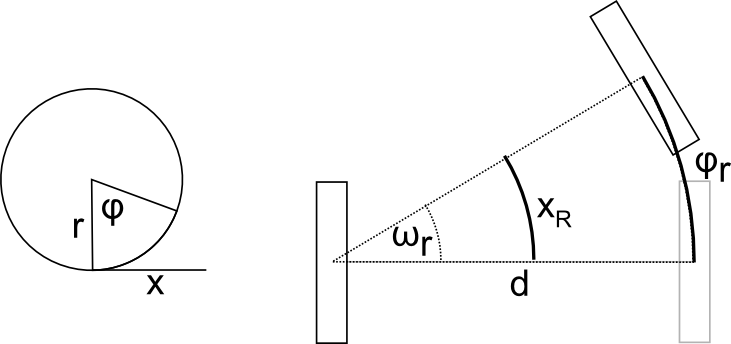
\includegraphics[width=0.9\textwidth]{figs/wheelrotation.png}
	% \caption{Left: Differential wheel robot pivoting around its left wheel. Right: A wheel with radius $r$ moves by $\phi r$ when rotated by $\phi$ degrees.}
	\caption{Left:差速轮机器人围绕其左轮转动。 右:旋转$ \phi $度时,半径为$ r $的车轮由$ \phi r $移动。}
	\label{fig:wheelrotation}
\end{figure}

% How each of the two wheels in our example contributes to the speed of the robot's center---where its coordinate system is anchored---requires the following trick: we calculate the contribution of each individual wheel while assuming all other wheels remaining un-actuated. In this example, the distance traveled by the center point is exactly half of that traveled by each individual wheel, assuming the non-actuated wheel rotating around its ground contact point (Figure \ref{fig:wheelrotation}). We can therefore write

在我们的例子中,两个车轮中的每一个如何有助于机器人中心的速度 - 其坐标系统被锚定 - 需要以下诀窍:我们计算每个车轮的贡献,同时假设所有其他车轮保持不变,动。 在这个例子中,由中心点行进的距离恰好是每个单独车轮行驶的距离的一半,假设非致动轮围绕其接地点旋转(图\ref {fig:wheelrotation})。 所以我们可以写

\begin{equation}
\dot{x_R}=\frac{r\dot{\phi_l}}{2}+\frac{r\dot{\phi_r}}{2}
\end{equation}
% given the speeds $ \dot{\phi_l}$ and $ \dot{\phi_r}$ of the left and the right wheel, respectively.

给定左右车轮的$ \dot {\phi_l} $和$ \dot {\phi_r} $的速度。

\begin{framed}
% Think about how the robot's speed along its y-axis is affected by the wheel-speed given the coordinate system in the drawing above. Think about the kinematic constraints that the standard wheels impose.
想想如上图所示的坐标系,机器人沿其y轴的速度如何受到车轮速度的影响。 考虑标准车轮施加的运动学约束。
\end{framed}

% Hard to believe at first, but the speed of the robot along its y-axis is always zero. This is because the constraints of the standard wheel tell us that the robot can never slide.  We are now left with calculating the rotation of the robot around its z-axis. That there is such a thing can be immediately seen when imaging the robot's wheels spinning in opposite directions. We will again consider each wheel independently. Assuming the left wheel to be non-actuated, spinning the right wheel forwards will lead to counter-clockwise rotation. Given an axle diameter (distance between the robot's wheels) $ d$, we can now write

首先很难相信,但机器人沿其y轴的速度总是为零。 这是因为标准轮的限制告诉我们,机器人永远不会滑动。 我们现在离开计算机器人围绕其z轴的旋转。 当成像机器人的轮子在相反方向旋转时,可以立即看到这样的事情。 我们将再次考虑每个轮子。 假设左轮未被致动,则向右旋转右轮将导致逆时针旋转。 给定轴直径(机器人轮子之间的距离)$ d $,我们现在可以写

\begin{equation}
\omega_r d = \phi_r r
\end{equation}
% with $ \omega_r$ the angle of rotation around the left wheel (Figure \ref{fig:wheelrotation}, right). Taking the derivative on both sides yields speeds and we can write

以$ \omega_r $为左轮的旋转角度(图\ref {fig:wheelrotation},右)。 取两边的衍生产生速度,我们可以写

\begin{equation}
\dot{\omega_r} = \frac{\dot{\phi_r} r}{d}
\end{equation}
% Adding the rotation speeds up (with the one around the right wheel being negative based on the right-hand grip rule), leads to

导致旋转速度加快(右侧车轮围绕右侧的车轮为负)

\begin{equation}
\dot{\theta}=\frac{\dot{\phi_r} r}{d}-\frac{\dot{\phi_l} r}{d}
\end{equation}

% Putting it all together, we can write
把它们放在一起,我们可以写

\begin{equation}\label{eq:diffwheels}
\left(\begin{array}{c} \dot{x_I}\\\dot{y_I}\\\dot{\theta}\end{array}\right)=\left(\begin{array}{ccc}
cos(\theta) & -sin(\theta) & 0 \\
sin(\theta) & cos(\theta) & 0 \\
0 & 0 & 1\end{array}\right)\left(\begin{array}{c}\frac{r\dot{\phi_l}}{2}+\frac{r\dot{\phi_r}}{2}\\0\\\frac{\dot{\phi_r} r}{d}-\frac{\dot{\phi_l} r}{d}\end{array}\right)
\end{equation}

% \subsubsection{From Forward Kinematics to Odometry}
\subsubsection{从正运动学到气压测量}
% Equation \ref{eq:diffwheels} only provides us with the relationship between the robot's wheel-speed and its speed in the inertial frame. Calculating its actual pose in the inertial frame is known as \emph{odometry}\index{Odometry}. Technically, it requires integrating (\ref{eq:diffwheels}) from 0 to the current time $T$. As this is not possible, but for very special cases, one can approximate the robot's pose by summing up speeds over discrete time intervals, or more precisely

方程式\ref {eq:diffwheels}仅为我们提供了机器人的轮速与惯坐标系中的速度之间的关系。 计算其在惯坐标系中的实际姿态称为\emph {odometry} \index {Odometry}。 从技术上讲,它需要从0到当前时间$ T $的集成(\ref {eq:diffwheels})。 由于这是不可能的,但是对于非常特殊的情况,可以通过在离散的时间间隔上求和速度来近似机器人的姿态,或者更准确地说

\begin{equation}
\left(\begin{array}{c} {x_I}(T)\\{y_I}(T)\\{\theta}(T)\end{array}\right)=
\int_0^T \left(\begin{array}{c} \dot{x_I}(t)\\\dot{y_I}(t)\\\dot{\theta}(t)\end{array}\right) dt \approx 
\sum_{k=0}^{k=T}\left(\begin{array}{c} \Delta{x_I}(k)\\\Delta{y_I}(k)\\\Delta{\theta}(k)\end{array}\right)\Delta t
\end{equation} which can be calculated incrementally as
\begin{equation}\label{eq:odometry}
x_I(k+1)=x_I(k)+\Delta x (k)
\end{equation}
% using $\Delta x(k) \approx \dot{x_I}(t)$ and similar expressions for $y_I$ and $\theta$. Note that (\ref{eq:odometry}) is just an approximation. The larger $\Delta t$ becomes, the more inaccurate this approximation becomes as the robot's speed might change during the interval.   

使用$ \Delta x(k)\approx\dot {x_I}(t)$和$ y_I $和$ \theta $的类似表达式。 注意(\ref{eq:odometry})只是一个近似值。 较大的$ \Delta t $变为,随着机器人的速度在间隔期间可能改变,该近似变得越不准确。

\begin{framed}
% Don't let the notion of an integral worry you! As robots' computers are fundamentally discrete, integrals usually turn into sums, which are nothing than for-loops.

不要让一个整体的概念担心你! 由于机器人的计算机基本上是离散的,所以积分通常变成和,这不是for循环。
\end{framed}



% \subsection{Forward kinematics of Car-like steering}
\subsection{汽车转向的正运动学}
% Differential wheel drives are very popular in mobile robotics as they are very easy to build, maintain, and control. Although not holonomic, a differential drive can approximate the function of a fully holonomic robot by first driving on the spot to achieve the desired heading and then driving straight. Drawbacks of the differential drive are its reliance on a caster wheel, which performs poorly at high speeds, and difficulties in driving straight lines as this requires both motors to drive at the exact same speed.

差速轮驱动器在移动机器人中非常受欢迎,因为它们非常易于构建,维护和控制。 虽然不完整,但是差速驱动器可以通过首先在现场驾驶以实现所需的航向,然后直线行驶,来逼近完全整体的机器人的功能。 差速驱动器的缺点在于其依赖于脚轮速度较差的脚轮,以及驱动直线的困难,因为这要求电机以完全相同的速度驱动。

% These drawbacks are mitigated by car-like mechanisms, which are driven by a single motor and can steer their front wheels. This mechanism is known as ``Ackermann steering'' \index{Ackermann steering}. Ackermann steering should not be confused with ``turntable'' steering \index{Turntable steering} where the front wheels are fixed on an axis with central pivot point. Instead, each wheel has its own pivot point and the system is constrained in such a way that all wheels of the car drive on circles with a common center point, avoiding skid. As the Ackermann mechanism lets all wheels drive on circles with a common center point, its kinematics can be approximated by those of a tricycle with rear-wheel drive, or even simpler by a bicycle. This is shown in Figure \ref{fig:ackermann}.

这些缺点通过由单个电动机驱动并且可以引导其前轮的类似汽车的机构来减轻。 这种机制被称为“Ackermann转向”\index{Ackermann转向}。 Ackermann转向不应与“转盘”转向\index{转盘转向}混淆,前轮固定在具有中心枢轴点的轴上。 相反,每个车轮都有自己的枢轴点,并且系统受到限制,使得汽车的所有轮子都具有共同的中心点的圆圈,避免了滑动。 由于Ackermann机构使所有车轮都能在具有共同中心点的圆圈上行驶,所以其运动学可以由具有后轮驱动的三轮车的运动学近似,或者甚至由自行车更简单。 这显示在图\ref {fig:ackermann}中。

\begin{figure}[htb!]
	\centering
		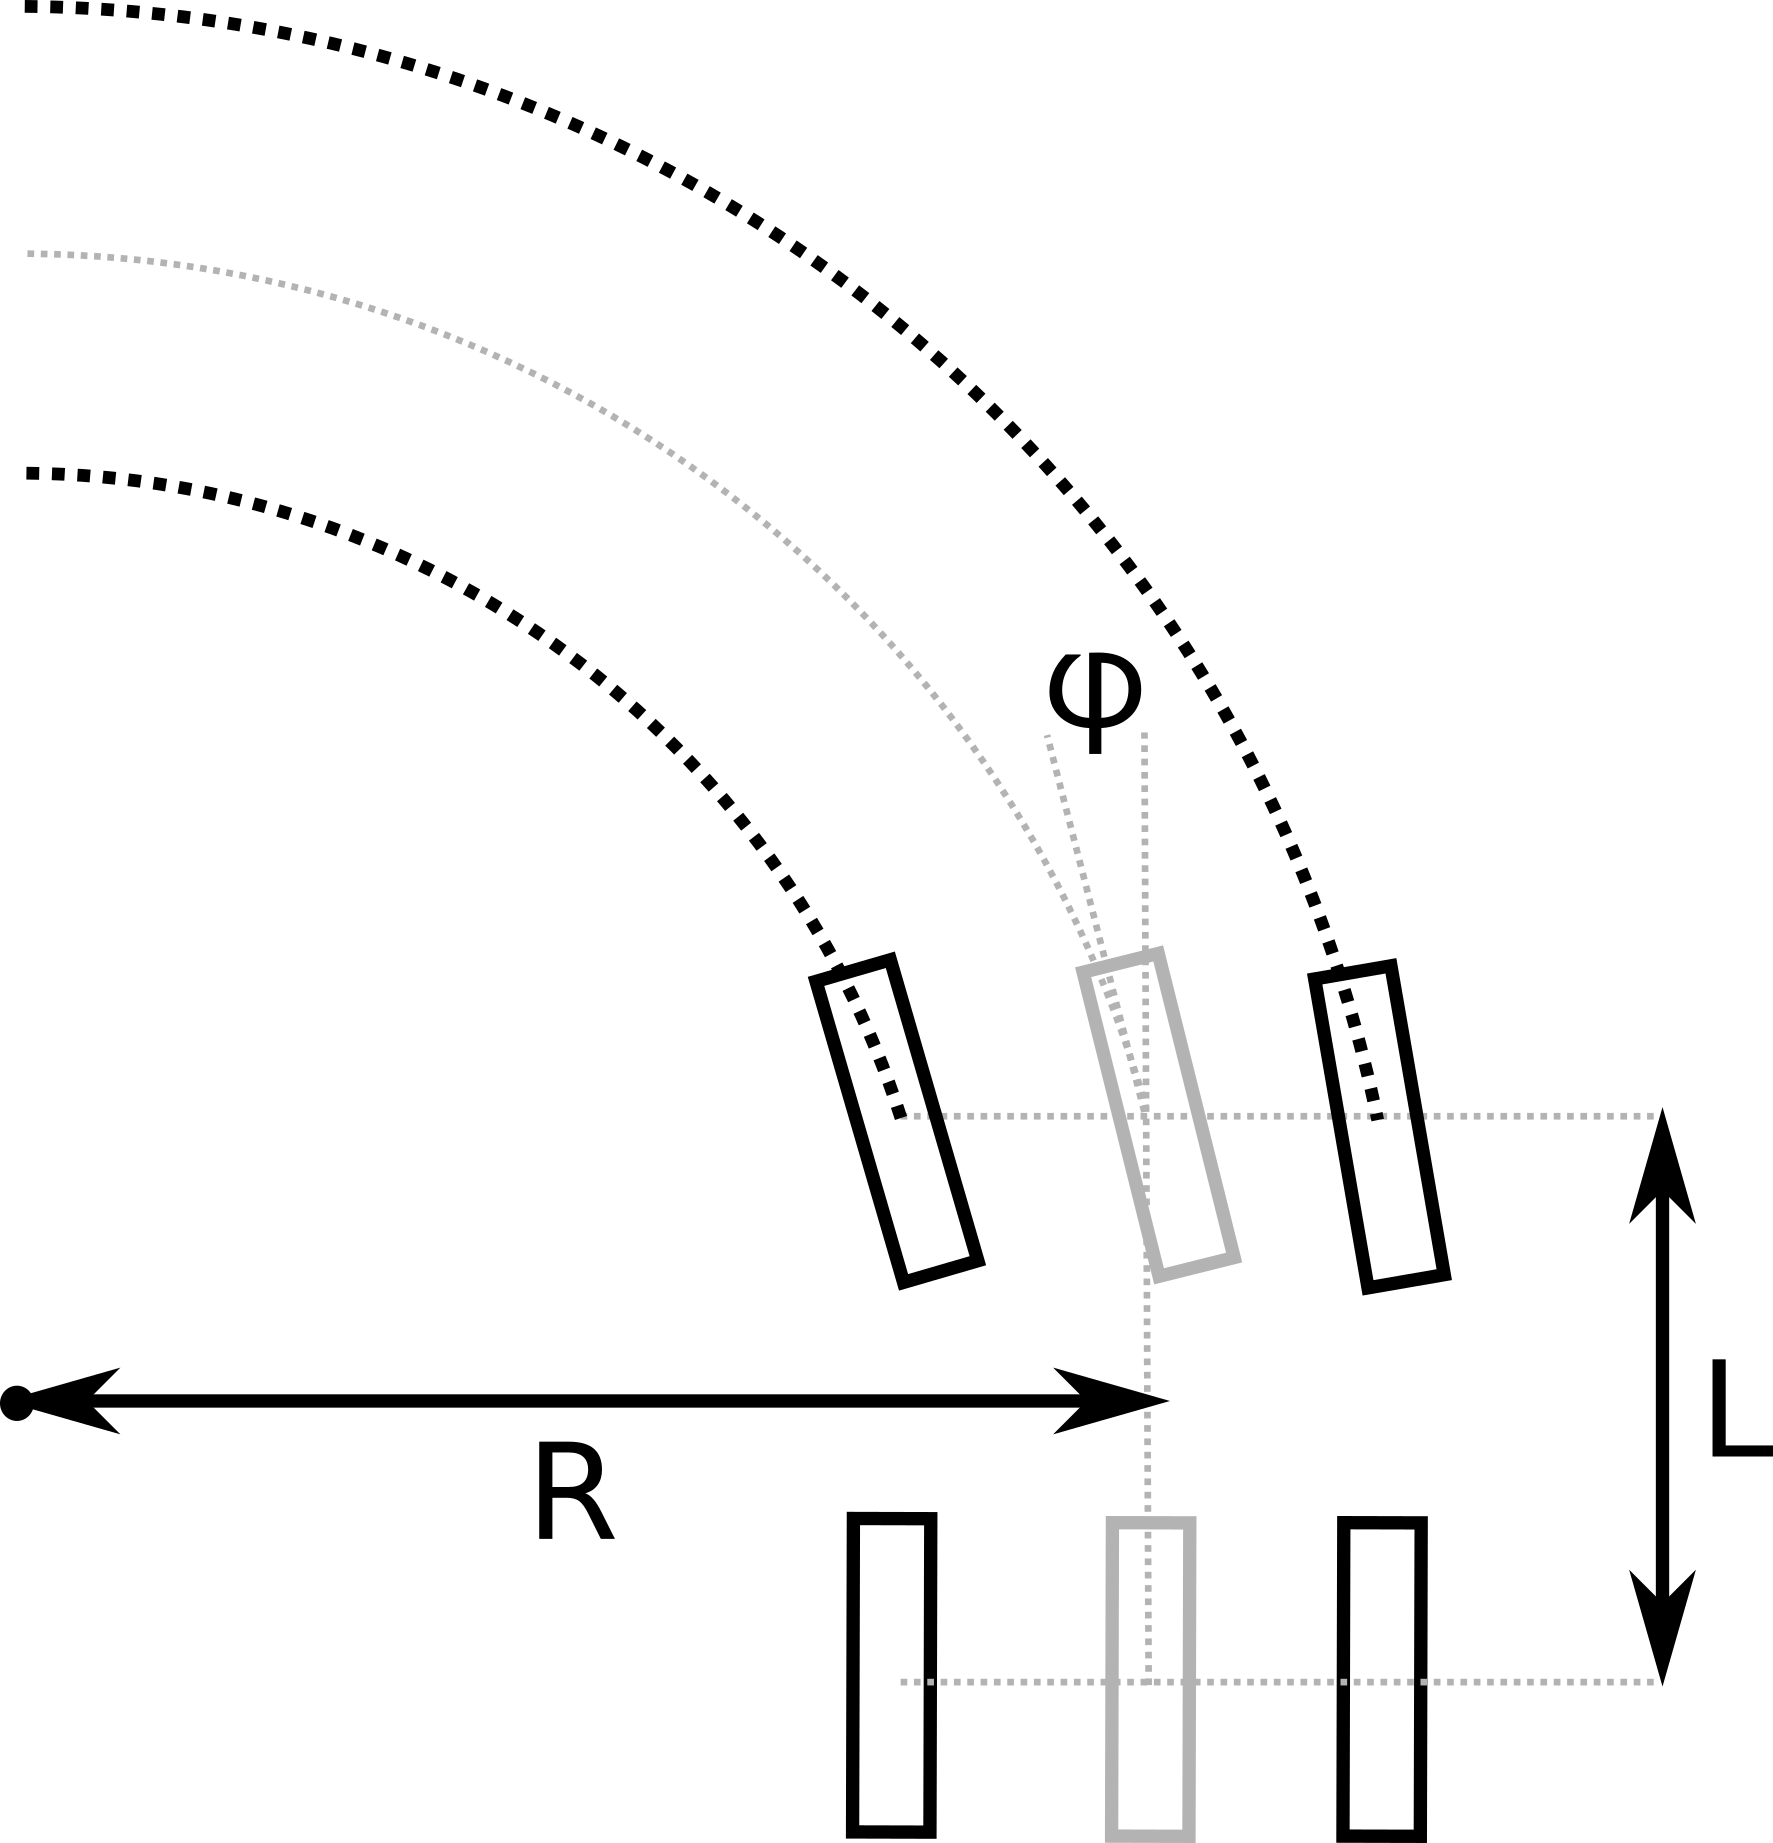
\includegraphics[width=0.9\textwidth]{figs/ackermann.png}
	% \caption{Left: Kinematics of car-like steering and the equivalent bicycle model. Right: Mechanism of an Ackermann vehicle.}
	\caption {Left:车载转向的运动学和等效的自行车模型。 权利:Ackermann车辆的机制。}
	\label{fig:ackermann}
\end{figure}

% Let the car have the shape of a box with length $L$ between rear and front axis. Let the center point of the common circle described by all wheels be distance $ R$ from the car's longitudinal center line.  Then, the steering angle $ \phi$ is given by

让汽车的后部和前轴之间的长度为$ L $的盒子的形状。 让所有车轮描述的共同圆的中心点距离汽车纵向中心线的距离$ R $。 然后,转向角$ \phi $由...给出

\begin{equation}\label{eq:ackermann}
\tan \phi = \frac{L}{R}
\end{equation}

% The angles of the left and the right wheel, $ \phi_l$ and $ \phi_r$ can be calculated using the fact that all wheels of the car rotate around circles with a common center point. With the distance between the two front wheels $l$, we can write

左右轮的角度$ \phi_l $和$ \phi_r $可以使用汽车的所有轮子围绕具有公共中心点的圆周旋转的事实来计算。 两个前轮之间的距离$ l $,我们可以写

\begin{eqnarray}
\frac{L}{R-l/2}&=\tan{(\pi/2-\phi_r)}\\
\frac{L}{R+l/2}&=\tan{(\pi/2-\phi_l)}
\end{eqnarray}
% This is important, as it allows us to calculate the resulting wheel angles resulting from a specific angle $\phi$ and test whether they are within the constraints of the actual vehicle.

这很重要,因为它允许我们计算由特定角度$ \phi $产生的所得到的车轮角度,并测试它们是否在实际车辆的限制之内。

% Assuming the wheelspeed to be $\dot{\omega}$ and the wheel radius $r$, we can calculate the speeds in the robot's coordinate frame to

假设车轮速度为$ \dot {\omega} $和车轮半径$ r $,我们可以计算机器人坐标系中的速度

\begin{eqnarray}
\dot{x}_r=\dot{\omega}r\\
\dot{y}_r=0\\
\dot{\theta}_r=\frac{\dot{\omega}r\tan\phi}{L}
\end{eqnarray}
% using (\ref{eq:ackermann}) to calculate the circle radius $R$. 
使用(\ref {eq:ackermann})计算圆半径$ R $。

% \section{Forward Kinematics using the Denavit-Hartenberg scheme}
\section{使用Denavit-Hartenberg方案的前进运动学}

% So far, we have considered the forward kinematics of wheeled mechanisms and simple arms and derived relationships between actuator parameters and velocities using basic trigonometry. In the specific case of multi-link arms, we can also think about the forward kinematics as a chain of homogenous transformations with respect to a coordinate system mounted at the base of a manipulator or a fixed position in the room. Deriving these transformations can be confusing and can be facilitated by following a ``recipe'' such as conceived by Denavit and Hartenberg. The so-called Denavit-Hartenberg (DH) \index{Denavit-Hartenberg parameters}scheme has evolved as quasi-standard and can easily be automatized, i.e., applied to a 3D model of a robotic arm, e.g. 

到目前为止,我们已经考虑了使用基本三角法的轮式机构和简单臂的正运动学和致动器参数和速度之间的导出关系。 在多连杆臂的具体情况下,我们还可以将正运动学视为相对于安装在机械手的基座或房间中固定位置的坐标系的均匀变换链。 导出这些转换可能会令人困惑,并且可以通过遵循由“Denavit”和“Hartenberg”构思的“配方”来促成这些转换。 所谓的Denavit-Hartenberg(DH)\index {Denavit-Hartenberg参数}方案已经演变为准标准,并且可以容易地自动化,即应用于机器人臂的3D模型,例如,

% A manipulating arm consists of links that are connected by joints. Joints can be either rotational or prismatic, i.e., change their length and thus providing additional degrees of freedom. Knowing the length of all rigid links, the position of the manipulators end-effector is fully described by its joint angles and joint offset (for prismatic joints).

操纵臂由通过接头连接的连杆构成。 接头可以是旋转的或棱柱形的,即改变其长度,从而提供额外的自由度。 知道所有刚性连杆的长度,操作臂末端驱动的位置通过其关节角度和关节偏移量完全描述(用于棱柱形接头)。

%% Was Commented
%In industrial manipulators, the number of joints is usually equal to the degrees of freedom of the manipulator. As most manipulators are holonomic, the forward kinematics allow you---unlike on non-holonomic wheeled platforms---to directly relate absolute positions of joints with absolute positions in Cartesian space. It is also possible to derive equations that relate the speed of the joints to speed in Cartesian space. Like for wheeled platforms, this can be achieved via a Jacobian matrix.  At certain positions, the mapping provided by the Jacobian is not invertible, i.e., some velocities in Cartesian space are unachievable. These points are called singularities.
%% Was Commented

\screencast{http://youtu.be/rA9tm0gTln8}{denavithartenberg}
% In oder to use the DH-convention, we first need to define a coordinate system at each joint. We chose the z-axis to be the axis of rotation for a hinge joint and the axis of translation for a prismatic joint. We can now find the common normal between the z-axes of two subsequent joints, i.e., a line that is orthogonal to each z-axis and intersects both. With the direction of the x-axis at the base arbitrary, subsequent x-axis are chosen such that they lie on the common normal shared between two joints. Whereas the direction of the z-axis is given by the positive direction of rotation (right hand rule), the x-axis points away from the previous joint. This allows defining the y-axis using the right-hand rule. Note that these rules, in particular the requirement that $x$-axes lie along the commom normal, might result in coordinate systems with their origins outside the joint. %Rather, the origin of joint $n$ is at the intersection of 

为了使用DH约定,我们首先需要在每个关节定义一个坐标系。 我们选择z轴为铰链接头的旋转轴线和棱柱形接头的平移轴。 我们现在可以找到两个后续关节的z轴之间的共同法线,即与每个z轴正交并且与两个相交的线。 随着x轴方向在任意的底部,随后的x轴被选择为使它们位于两个关节之间共同的公共正常上。 而z轴的方向由正旋转方向(右手规则)给出,x轴指向远离前一关节。 这允许使用右手规则来定义y轴。 请注意,这些规则,特别是$ x $ -axes沿着commom正常的要求可能会导致坐标系统的起源在关节之外。 

% The transformation between two joints is then fully described by the following four parameters:

然后通过以下四个参数充分描述两个关节之间的转换:

% \begin{enumerate}
% \item The length $ r$ of the common normal between the $z$-axes of two joints $i$ and $i-1$ (link length).
% \item The angle $ \alpha$ between the z-axes of the two joints with respect to the common normal (link twist), i.e., the angle between the old and the new $z$-axis, measured about the common normal.
% \item The distance $d$ between the joint axes (link offset), i.e., the offset along the previous $z$-axis to the common normal.
% \item The rotation $ \theta$ around the common axis along which the link offset is measured (joint angle), i.e., the angle from the old $x$-axis to the new $x$-axis, about the previous $z$-axis.
% \end{enumerate}

\begin{enumerate}
\item 两个关节的$ z $ -axes $ i $和$ i-1 $(链接长度)之间的常用法线的长度$ r $。
\item 相对于公共正常(链接扭曲)的两个关节的z轴之间的角度$ \alpha $,即关于普通法线测量的旧和新$ z $ -axis之间的角度。
\item 关节轴(链接偏移)之间的距离$ d $,即前一个$ z $ -axis的偏移量与常规法线的距离。
\item 旋转$ \theta $围绕测量链接偏移的公共轴(关节角度),即从旧$ x $ -axis到新$ x $ -axis的角度,关于前一个$ z$轴。
\end{enumerate}

% Two of the D-H parameters describe the link between the joints, and the other two describe the link's connection to a neighboring link. Depending on the link/joint type, these numbers are fixed or can be controlled. For example, in a revolute joint $ \theta$ is the varying joint angle, while all other quantities are fixed.  Similarly, for a prismatic joint $ d$ is the joint variable. An example of two revolute joints is shown in Figure \ref{fig:denavit}.

两个D-H参数描述了关节之间的链接,另外两个描述了链路与相邻链路的连接。 根据链接/关节类型,这些数字是固定的或可以控制的。 例如,在旋转关节中,$ \theta$是变化的关节角度,而所有其他数量是固定的。 同样,对于一个棱柱关节,$ d $是关节变量。 两个旋转关节的例子如图\ref {fig:denavit}所示。

\begin{figure}
	\centering
		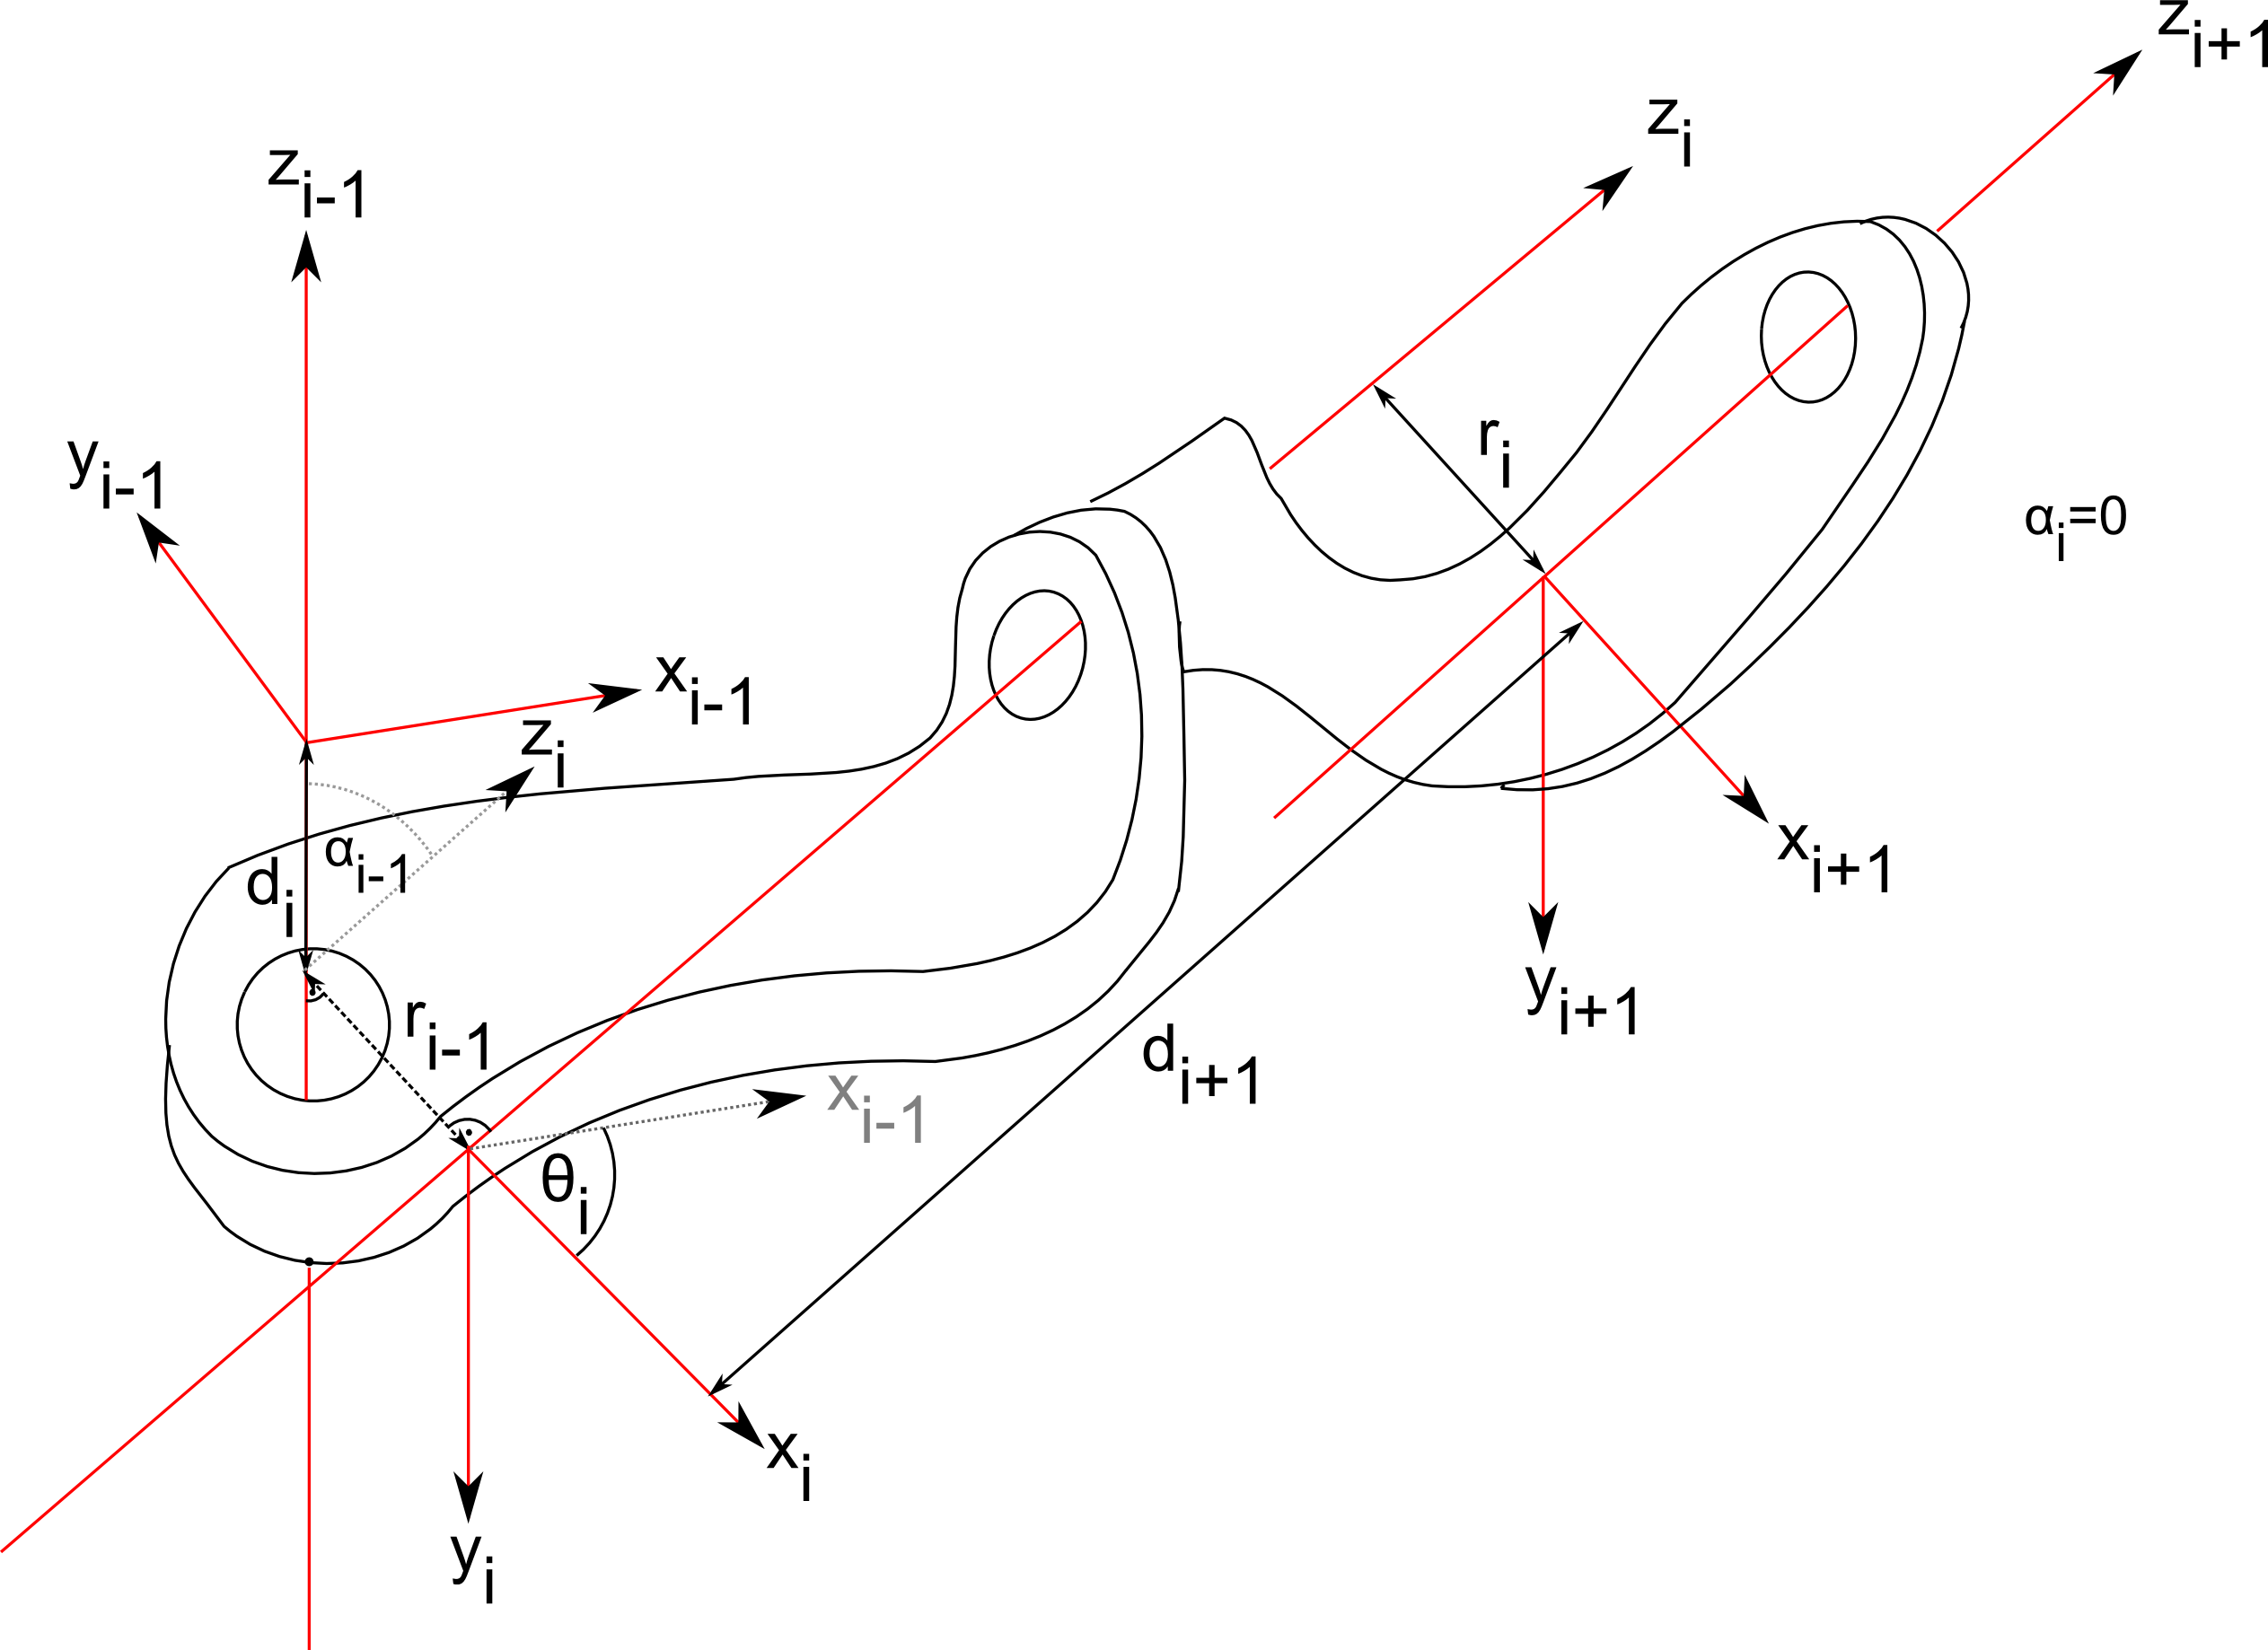
\includegraphics[width=\textwidth]{figs/denavit-hartenberg}
	% \caption{Example of selected Denavit-Hartenberg parameters for three revolute joints. The z-axes of joint $i$ and $i+1$ are parallel.}
	\caption {三个旋转关节的选定的Denavit-Hartenberg参数的例子。 关节$ i $和$ i + 1$的z轴是并行的。}
	\label{fig:denavit}
\end{figure}



% The coordinate transform from one link ($ i-1$) to another ($i$) can now be constructed  using the following matrix:

现在可以使用以下矩阵来构建从一个链接($ i-1 $)到另一个链接($ i $)的坐标变换:

\begin{eqnarray}{ll}
\nonumber
_{n-1}^nT=&
\left(
\begin{array}{ccc|c}
\cos \theta_n & -\sin \theta_n \cos\alpha_n & \sin\theta_n \sin\alpha_n & r_n \cos\theta_n\\
\sin \theta_n & \cos\theta_n \cos\alpha_n & -\cos\theta_n\sin\alpha_n & r_n \sin\theta_n\\
0 & \sin\alpha_n & \cos\alpha_n & d_n\\
\hline
0 & 0 & 0 & 1
\end{array}
\right)\\
&=
\left(
\begin{array}{c|c}
R & t\\
\hline
0 \quad 0 \quad 0 & 1
\end{array}
\right)
\end{eqnarray}
% with the rotation matrix $R$ and the translation vector $t$. This matrix can be constructed by a series of rotations and translations, one for each DH parameter:

旋转矩阵$ R $和翻译向量$ t $。 该矩阵可以通过一系列旋转和平移来构造,每个DH参数一个:

\begin{equation}
_{n-1}^nT=T_z'(d_n)\dot R_z'(\theta_n) \dot T_x(r_n) \dot R_x(\alpha_n)
\end{equation}
with
\begin{equation}
T_z'(d_n)=
\left(
\begin{array}{ccc|c}
1 & 0 & 0 & 0\\
0 & 1 & 0 & 0\\
0 & 0 & 1 & d_n\\
\hline
0 & 0 & 0 & 1
\end{array}
\right)
\enskip
R_z'(\theta_n)=\left(
\begin{array}{ccc|c}
\cos\theta_n & -\sin\theta_n & 0 & 0\\
\sin\theta_n & \cos\theta_n & 0 & 0\\
0 & 0 & 1 & 0\\
\hline
0 & 0 & 0 & 1
\end{array}
\right)
\end{equation}
and
\begin{equation}
T_x(r_n)=
\left(
\begin{array}{ccc|c}
1 & 0 & 0 & r_n\\
0 & 1 & 0 & 0\\
0 & 0 & 1 & 0\\
\hline
0 & 0 & 0 & 1
\end{array}
\right)
\enskip
R_x(\alpha_n)=\left(
\begin{array}{ccc|c}
1 & 0 & 0 & 0\\
0 & \cos\alpha_n & -\sin\alpha_n & 0\\
0 & \sin\alpha_n & \cos\alpha_n & 0\\
\hline
0 & 0 & 0 & 1
\end{array}
\right)
\end{equation} 
% These are a translation of $d_n$ along the previous z-axis ($T_z'(d_n)$), a rotation of $\theta_n$ about the previous z-axis ($R_z'(\theta_n)$), a translation of $r_n$ along the new $x$-axis ($T_x(r_n)$)and a rotation of $\alpha_n$ around the new $x$-axis ($R_x(\alpha_n)$).

这些是前一个z轴($ T_z'(d_n)$)的$ d_n $,前一个z轴($ R_z'(\theta_n)$)的$ \theta_n $的旋转,翻译 在新的$ x $ -axis($ T_x(r_n)$)之间的$ r_n $和新的$ x $ -axis($ R_x(\alpha_n)$)周围的$ \alpha_n $的旋转。

% Like for any homogeneous transfrom, the inverse $_{n-1}^nT^{-1}n$ is given by

像任何均匀变换一样,逆$ _ {n-1} ^ nT ^ { - 1} n $由给出

\begin{equation}
^{n-1}_nT=\left(
\begin{array}{c|c}
R^{-1} & -R^{-1}T\\
\hline
0 \quad 0 \quad 0 \quad 1
\end{array}
\right)
\end{equation}
% with the inverse of $R$ simply being its transpose.
与$ R $的倒数只是其转置。
